\documentclass[review]{elsarticle}

\usepackage{lineno,hyperref,ulem,todonotes}
\usepackage{rotating}
\usepackage{amsmath}
\modulolinenumbers[5]
%\usepackage{natbib}
%\journal{Journal of \LaTeX\ Templates}

%%%%%%%%%%%%%%%%%%%%%%%
%% Elsevier bibliography styles
%%%%%%%%%%%%%%%%%%%%%%%
%% To change the style, put a % in front of the second line of the current style and
%% remove the % from the second line of the style you would like to use.
%%%%%%%%%%%%%%%%%%%%%%%

%% Numbered
\bibliographystyle{model1-num-names}

%% Numbered without titles
%\bibliographystyle{model1a-num-names}

%% Harvard
%\bibliographystyle{model2-names.bst}\biboptions{authoryear}

%% Vancouver numbered
%\usepackage{numcompress}\bibliographystyle{model3-num-names}

%% Vancouver name/year
%\usepackage{numcompress}\bibliographystyle{model4-names}\biboptions{authoryear}

%% APA style
%\bibliographystyle{model5-names}\biboptions{authoryear}

%% AMA style
%\usepackage{numcompress}\bibliographystyle{model6-num-names}

%% `Elsevier LaTeX' style
%\bibliographystyle{elsarticle-num}
%%%%%%%%%%%%%%%%%%%%%%%

\begin{document}

\begin{frontmatter}

\title{An intermediate-scale model for thermal hydrology in low-relief permafrost-affected landscapes}

\author[ornl]{Ahmad Jan} \author[lanl]{Ethan T. Coon} \author[ornl]{Scott L. Painter} \author[lanl]{Rao Garimella} \author[lanl]{J. David Moulton}

\address[ornl]{Climate Change Science Institute and Environmental Sciences Division, Oak Ridge National Laboratory} 
\address[lanl]{Los Alamos National Laboratory} 

%\tnotetext[mytitlenote]{Fully documented templates are available in the elsarticle package on \href{http://www.ctan.org/tex-archive/macros/latex/contrib/elsarticle}{CTAN}.}

%% Group authors per affiliation:
%\author{Elsevier\fnref{myfootnote}}
%\address{Radarweg 29, Amsterdam}
%\fntext[myfootnote]{Since 1880.}

%% or include affiliations in footnotes:
%\author[mymainaddress,mysecondaryaddress]{Elsevier Inc}
%\ead[url]{www.elsevier.com}

%\author[mysecondaryaddress]{Global Customer Service\corref{mycorrespondingauthor}}
%\cortext[mycorrespondingauthor]{Corresponding author}
%\ead{support@elsevier.com}

%\address[mymainaddress]{1600 John F Kennedy Boulevard, Philadelphia}
%\address[mysecondaryaddress]{360 Park Avenue South, New York}

\begin{abstract}
Integrated surface/subsurface models for simulating the thermal hydrology of permafrost-affected regions in a warming climate have recently become available, but computational demands of those new process-rich simulation tools have thus far limited their applications to one-dimensional or small two-dimensional simulations. 
We present a mixed-dimensional model structure for efficiently simulating surface/subsurface thermal hydrology in low-relief permafrost regions at watershed scales. The approach solves an operator-split system, sequentially coupling a two-dimensional surface thermal hydrology system with a family of one-dimensional vertical columns, where each column represents a fully coupled surface/subsurface thermal hydrology system without lateral flows. The overland thermal hydrology system with no sources acts to redistribute mass and energy horizontally by updating the column systems before they advance in time. We show that the approach is highly scalable, supports subcycling of different processes, and compares well with the corresponding fully three-dimensional representation at significantly less computational cost. These advances enable state-of-the-art representations of freezing soil physics to be coupled with thermal overland flow and surface energy balance at scales of 100s of meters. Although developed and demonstrated for permafrost thermal hydrology, the mixed-dimensional model structure is applicable to integrated surface/subsurface thermal hydrology in general. 
\end{abstract}

\begin{keyword}
Mixed-dimensional model\sep Permafrost thermal hydrology  \sep Integrated surface/subsurface flow modeling \sep Arctic 
%\MSC[2010] 00-01\sep  99-00
\end{keyword}
\end{frontmatter}

\linenumbers

\section{Introduction}

Approximately 23\% of the land surface in the Northern Hemisphere is underlain by continuous permafrost (91-100\% frozen area), and another 17\% is occupied by discontinuous permafrost (50-90\% frozen area)~\cite{brown1997circum,jorgenson2001permafrost}. A massive amount of organic carbon is stored in those regions \cite{schuur2015climate,bg-11-6573-2014}, which are warming at a rate considerably faster than the rest of the planet~\cite{turner2007arctic, hansen1999giss, assessment2004impacts}.  As the soils in that region warm, they have the potential to transform from a net sink to a net source of carbon to the atmosphere, which could increase the concentration of carbon in the atmosphere and in turn lead to further increase in the temperature~(e.g. \cite{koven2011permafrost}). Further, thawing and the resulting degradation of permafrost can cause significant changes in the surface and subsurface thermal hydrology and eventually can substantially alter the Arctic tundra ecosystems~\cite{osterkamp1983response, walvoord2007increased, lyon2009estimation, pachauri2014climate,koven2013analysis}. 

Those potential impacts and feedbacks in the terrestrial Arctic have motivated the development of increasingly sophisticated tools for simulating permafrost dynamics in a warming climate. Such simulations can help to better understand the consequences of soil warming and responses of tundra ecosystems to warming trends, and further expose the effects of permafrost degradation on surface and subsurface thermal hydrology. However, simulating permafrost dynamics in a complex and coupled surface/subsurface thermal hydrological environment is a challenging task, especially at larger spatiotemporal scales~\cite{painter2013modeling}.  A comprehensive review of the modeling efforts of the surface and subsurface can be found in~\cite{kurylyk2014climate}. Early research efforts focused on one-dimensional simulations for fundamental understanding of infiltration in cold climates; see, for example,~\cite{harlan1973analysis, guymon1974coupled, taylor1978model}. Similar one-dimensional approximations have been adopted as coarse-scale models in global land surface models \cite{takata2003development, nicolsky2007improved, lawrence2012simulation, koven2013analysis}.  Two-dimensional simulations with simplified physics (i.e. saturated conditions, subsurface only) have been used for understanding evolution of field-scale groundwater systems~\cite{mckenzie2007groundwater, bense2009evolution}, but do not represent key unsaturated zone processes that are needed to understand active layer dynamics and decomposition of soil organic matter.   It is worth pointing out that mathematical models with limited complexity, reduced dimensionality, and relatively coarse spatial resolutions provide some insight into permafrost dynamics but fail to represent important processes such as cryosuction, lateral surface and subsurface flows, and advective heat transfers. Simulations with more mechanistic representations of surface and vadose zone process in three-dimensions are essential to accurately capture the potential impacts of permafrost thawing on the surface and subsurface thermal hydrology and the resulting effects on the carbon cycle. 

Two- and three-dimensional models with explicit physics-based representations of ice/liquid/gas partitioning in the vadose zone~\cite{painter2014constitutive} have only recently started to appear. Painter [\citeyear{marsflo}] developed the three-phase, two-component model MarsFlo which has been used in Mars \cite{grimm2009mars} and Earth permafrost studies \cite{frampton2011}.  Karra et al. [\citeyear{karra2014three}] simplified that subsurface freezing-soil thermal hydrology representation by ignoring gas advection and implemented that Richards-like approximation in the highly parallel PFLOTRAN \cite{pflotran-web-page} code. Those computer codes are all subsurface-only models; that is, they do not represent surface flows and surface energy balance. Painter et al. \citeyear{spainter2016integrated} recently introduced the Arctic Terrestrial Simulator, which uses a sophisticated multiphysics management framework \cite{ecoon2016managing} to couple the three-dimensional subsurface representation of \cite{karra2014three} with a two-dimensional non-isothermal surface flow model, surface energy balance with and without snow, and a simple snow distribution model. 

Despite the significant progress in developing integrated surface/subsurface permafrost thermal hydrology models, significant challenges remain in moving to climate-relevant spatiotemporal scales. One of the challenges is that the integrated system is numerically stiff because of the highly dynamic surface system~\cite{spainter2016integrated} and the ice-liquid phase transition~\cite{dall2011robust}, which often results in relatively small time steps to achieve convergence. Small time steps are not problematic in one-dimensional simulations because a well-designed simulation tool will recover the time step quickly after a convergence failure. However, a small time step becomes problematic in large three-dimensional runs because it becomes increasingly likely that, at any given time, at least one computational cell will be experiencing a phase change and thus a small time step. The other major challenge is tracking thaw-induced subsidence. Traditional hydrological simulators are mainly designed to conduct three-dimensional simulations, however, deformations in a three-dimensional simulation are not easy to track due to mesh tangling and can be computationally expensive; further, poor mesh quality may raise questions about the accuracy of the results. 

To address the aforementioned challenges, we present a mixed-dimensional modeling strategy for process-rich simulations of integrated surface and subsurface thermal hydrology in tundra systems with low topographic gradients. The approach is intended for spatial scales intermediate between microtopography-resolving fine-scale simulations and the scale of an Earth system model grid cell. We demonstrate with simulations of polygonal tundra, large and carbon-rich regions of northern Siberia, Alaska, and Canada where soil cracking has led to the formation of subsurface ice wedges that honeycomb the subsurface and tesselate the land surface into polygonal patterns. Rather than solve a fully three-dimensional subsurface system tightly coupled to surface processes as in~\cite{spainter2016integrated}, we take advantage of physical insights gained from fine-scale simulations and approximate the integrated surface/subsurface dynamics with mutually independent 1-D columns, each associated with an ice wedge polygon. The columns are then sequentially coupled to a surface thermal flow system, solving the surface problem in an operator-split manner. This mixed-dimensional modeling approach is motivated by fine-scale simulations at the ice-wedge polygon scale that showed that differences in the thermal conditions among centers, rims and troughs of ice-wedge polygons are largely equilibrated by lateral heat transport during summer such that the system behaves similarly to a one-dimensional system on seasonal time scales. Mixed-dimensional model structures have been used previously in simulations of variably saturated flow at watershed scales, in particular to couple multiple 1-D unsaturated (vadose) zone representations to a two- or three-dimensional saturated zone; for example see~\cite{pikul1974numerical,zhu2011method,hybrid3D}. Here we apply the mixed-dimensional model structure to an integrated surface/subsurface flow system including surface and subsurface thermal processes and evaluate the accuracy and computational advantages of the approximation. 

%In addition to enabling process rich simulations at climate relevant scales, this work also demonstrates how advanced software design, in particular a configurable system for managing multiphysics simulations~\cite{ecoon2016managing}, can facilitate the implementation of models with novel spatial structures that take advantage of the physical insights of domain specialists but are difficult to express in conventional software. 



The paper is organized as follows: Section~\ref{arcos-framework} highlights the Advanced/Arctic  Terrestrial Simulator (ATS) and the Arcos multiphysics management framework, within which we implemented our approach. Section~\ref{motivation} presents some fine-scale simulation results and analysis that motivated the approach.  In Section~\ref{mixed-dim-model} we introduce our mixed-dimensional modeling approach, loosely coupled scheme and the ATS refactoring strategy. To illustrate the performance and efficiency of our modeling strategy, in Section~\ref{numerical-tests} we compare our numerical results with the three-dimensional simulations based on strong coupling, and present speedup and scalability of the new technique. Concluding remarks and future research are offered in Section~\ref{conclusion}.

\section{The ATS Software}\label{arcos-framework}

We implemented our mixed-dimensional modeling strategy in open-source parallel software known as Amanzi-ATS~\cite{ats-website} (or simply ATS). Amanzi-ATS is the result of extending the flow and reactive transport  simulator Amanzi~\cite{moulton2012high} by adding an advanced multiphysics management system known as Arcos~\cite{ecoon2016managing}. Arcos is key to managing the complex spatial structures used here. It was originally built to manage couplings among process models (denoted process kernels and abbreviated as PKs), which may be selected at runtime. A PK encapsulates the mathematical representation of a particular physical process or coupled set of processes; PKs are coupled together through Multiprocess Coordinators MPCs. An MPC is regarded as a PK by MPCs at higher levels in the tree, thus allowing complex hierarchical model structures to be built dynamically at runtime. In this work, we used Arcos to coordinate not only process kernels but also subdomains of the larger spatial domain. 

Amanzi, and by extension ATS, uses the Trilinos ~\cite{michael2003trilinos} framework for parallel infrastructure. An unstructured mesh framework \cite{garimella-2014-mstk} is included for interacting with the computational mesh. General polyhedral meshes are supported. Discretization accuracy is maintained on the potentially distorted grids through the use of the mimetic finite difference (MFD) method ~\cite{da2014mimetic, lipnikov2014mimetic}. The backward Euler method is used for time stepping with a Nonlinear Krylov Acceleration (NKA) method ~\cite{calef2013nonlinear, carlson1998design} to solve the resulting discretized residual equations. 

 The initialism ATS may refer to either the Advanced Terrestrial Simulator, which is the general capability, or the Arctic Terrestrial Simulator, which is one particular configuration~\cite{spainter2016integrated}, depending on context. The Arctic Terrestrial Simulator configuration solves strongly coupled surface energy balance, and surface and subsurface thermal hydrology with freeze/thaw dynamics. This work extends the ATS to work with a multicolumn spatial structure. 


\section{Motivation: Results from Fine-scale Simulations}\label{motivation}

This mixed-dimensional approach is motivated by the results of fine-scale, two-dimensional simulations on vertical cross-sections across ice-wedge polygons at the Barrow Environmental Observatory. The simulations coupled a surface energy balance model with and without snow, snow distribution models, models for thermal overland flow including phase change, and a recently developed three-phase subsurface thermal hydrology model. The soil properties were calibrated against borehole temperature data in a previous study~\cite{atchley2015}. The simulations were forced with meteorological data for the site. Those simulations used an unstructured mesh that conforms to surface topography derived from lidar measurements. Horizontal mesh resolution is approximately 0.25 m. Vertical resolution is 0.02 cm at the surface and gradually increases with depth. Details on boundary conditions and the spinup process can be found in \cite{spainter2016integrated}. 

Snapshots of ice and liquid saturation indices in cross-section across two ice-wedge polygons are shown in Fig.~\ref{oct15}. These snapshots are for October 15, 2013, which is during the fall freeze-up. During this period, the rims of the ice-wedge polygons are significantly colder than the centers and troughs because the thermally insulating snowpack is smaller on the rims. Previous one-dimensional simulations~\cite{atchley2016} have shown that thermal differences caused by differences in snow depth lead to differences in active layer thickness, the depth of the annual thaw. However, in the two-dimensional simulations shown here, the active layer thickness shows little variation across the polygon (Fig.~\ref{alt}). Although transient differences in subsurface temperature occur due to differences in snow depth, soil moisture content, and albedo, lateral heat transport is sufficient to equilibrate those differences by the time of maximum thaw. Thus, the active layer thickness, which is a primary control on the annual carbon decomposition rates, is not directly affected by microtopographic position within an ice-wedge polygon in cases where organic matter is relatively uniform. This lack of sensitivity suggests a model structure where the ice-wedge polygon becomes the unit computational cell on the surface. 

\begin{sidewaysfigure}[!htpb]
\centering
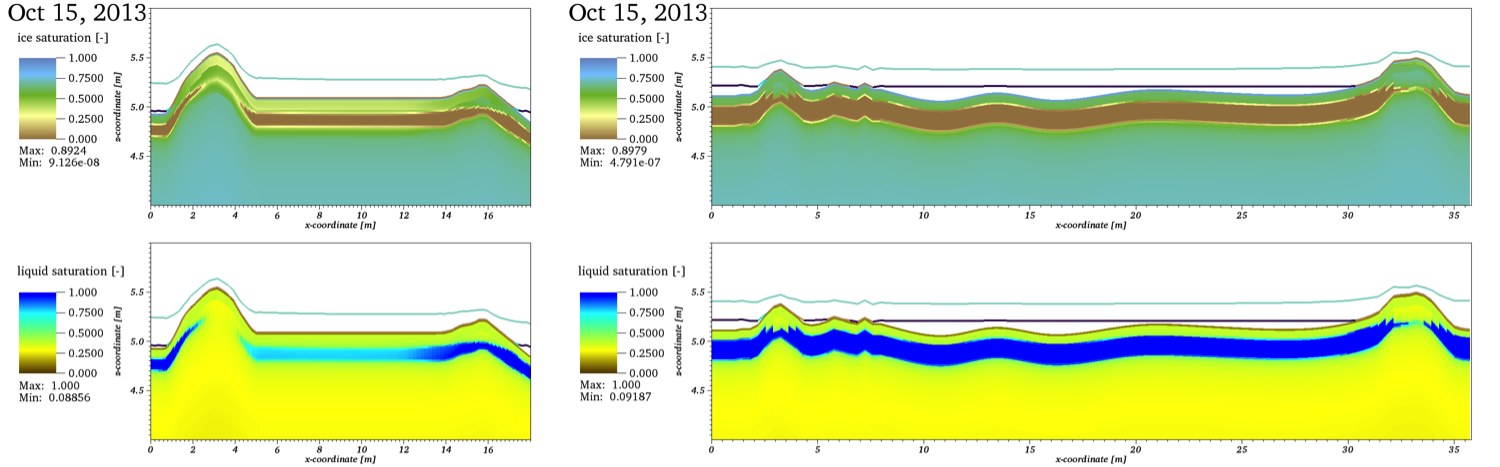
\includegraphics[height=8cm,width=17cm]{figures/FineScaleOct15.png}
\caption{Results from two-dimensional fine-scale modeling. Shown are snapshots of ice saturation index and liquid saturation index in cross-sections across two ice-wedge polygons.}
\label{oct15}
\end{sidewaysfigure}

\begin{figure}[!htpb]
\centering
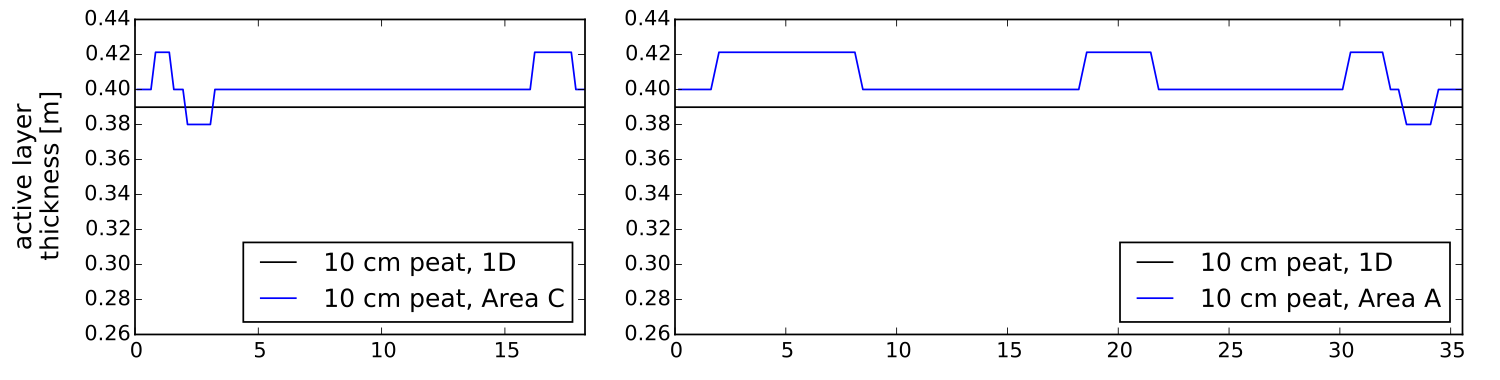
\includegraphics[height=5cm, width=12cm]{figures/ALT-finescale.png}
\caption{Active layer thickness from fine-scale modeling.  Note that the mesh resolution here is $2 cm$, and the discontinuities reflect jumps between cells of the mesh.}
\label{alt}
\end{figure}




\section{An Intermediate-scale Model}\label{mixed-dim-model}

Our intermediate-scale model has two components: a spatial structure that combines one-dimensional and two-dimensional domains, and an operator splitting scheme for coupling. We describe those aspects in this section followed by the 
 refactoring strategy of the ATS.
\subsection{Mixed-Dimensional Modeling Approach}

Our modeling strategy splits a 3D domain into $2N + 1$ subdomains, where $N$ is the total number of surface elements.  The workflow starts with a two-dimensional tessellation of the land surface, where each polygon in the surface mesh corresponds to an ice-wedge polygon. Standard mesh generation tools are then used to construct a 3D mesh by extruding each of the surface polygons vertically into the subsurface. This 3D mesh represents the entire domain of interest and is referred to as the primal mesh. Within ATS, the 3D primal mesh is then subdivided into $2N+1$ submeshes, where $N$ is the total number of surface elements. The total $2N+1$ subdomains include $N$ subdomains for 1D subsurface columns (on which flow and energy equations are solved), $N$ subdomains as the surface of those columns (on which surface water and energy storage is tracked along with a surface energy balance calculation), and one subdomain for the 2D overland system, on which lateral surface flow is solved.  To avoid confusion, hereafter the 2D overland system is referred to as surface$^*$ system, and the surface cell of each 1D columns will be called a surface system. The 1D columns and surface* system are highlighted in Fig.~\ref{surf-cols}. Arcos represents physics on these domains as a hierarchical PK tree which shows how the processes are coupled on and across these domains, as illustrated in Fig.~\ref{pk-tree}. The PK tree consists of individual conservation equations, strong (globally implicit) couplers, and weak (sequential) couplers highlighted in blue, light cyan, and orange colors, respectively. In our approach, the interaction at the interface between the surface* and 1D columns happens at the top level weak MPC. The strong MPC (on the left at the second level) is the surface* system. The weak MPC at the second level iterates over all the surface and subsurface subdomains. The PK-I, I $=1,2,3, \dots, N$ denote integrated surface (a cell) and subsurface (1D column) system. The tree attached to the black octagon shape is replicated across all PK-I, I $=1,2,3, \dots, N$.

\begin{figure}[!htpb]
\centering
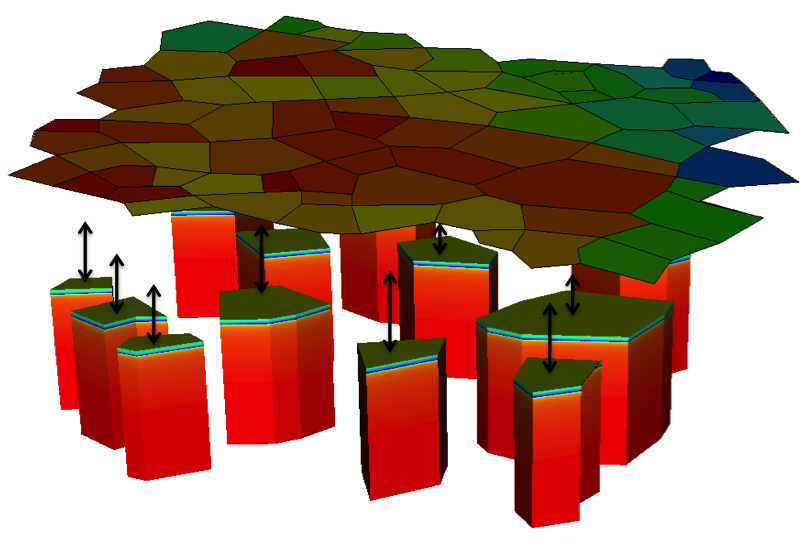
\includegraphics[height = 7.5cm, width=10cm]{figures/mixed-dim-model.png}
\caption{An illustration of the independent 1D subsurface columns coupled to the surface* system. The surface system (1D cells lying on the top of corresponding columns) are not shown.}
\label{surf-cols}
\end{figure}


\begin{figure}[!htpb]
\centering
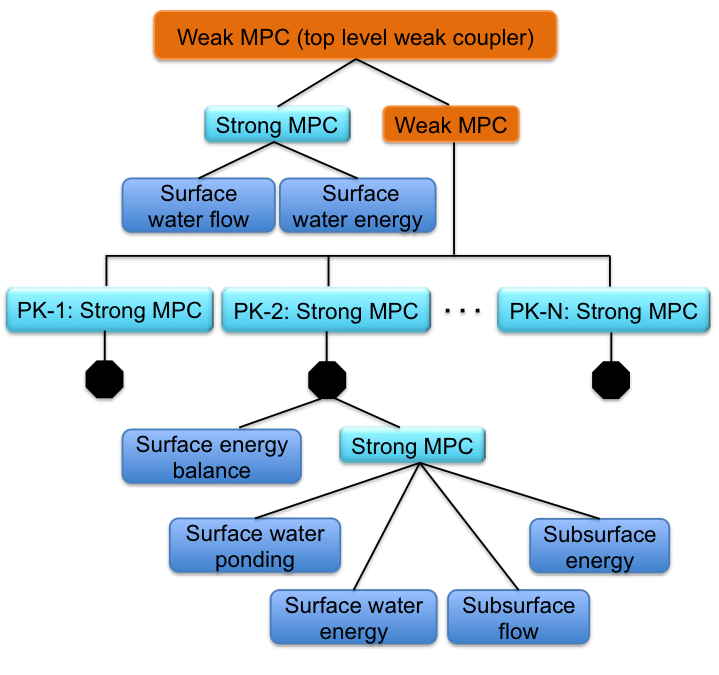
\includegraphics[height = 7.5cm, width=11cm]{figures/process-tree1.png}
\caption{A customized hierarchical structure of the process kernels. Blue blocks highlights independent process models; Light blue blocks strongly coupled independent process kernels; Orange blocks represent weak couplers.}
\label{pk-tree}
\end{figure}


\subsection{Operator Splitting Scheme}
The operator splitting scheme for advancing our mixed-dimensional model is a two-step sequential algorithm. First, we solve the surface* thermal hydrology system without any external or exchanged sources and then compute the solution of the one-dimensional columns. Each 1D column is a system of the subsurface thermal hydrology, surface ponding and energy exchange but no lateral flow, and surface energy balance. The first step mainly acts as a spatial distributor of the mass and energy. That is, it distributes the water and energy across the 2D overland system, and its solution serves as initial condition for the second step. After the update from the first step, we solve the family of 1D columns, and use the output of that half-step to update the surface* pressure and temperature for the next iteration in the algorithm. As depicted in Fig.~\ref{coupling-schematic}, the top and bottom orange spots represent 2D surface* system and 1D columns, respectively, and the cyan colors (in the middle) are intermediate steps for updating surface* and 1D column systems. For the sake of clarity, we will refer to the pressure and temperature fields of the first step as surface* pressure and temperature, while that of the second step will be called as subsurface and surface pressures and temperatures.


%\textbf{Refer to some published work related to mixed-dimensional modeling.}

\begin{figure}[h]
\centering
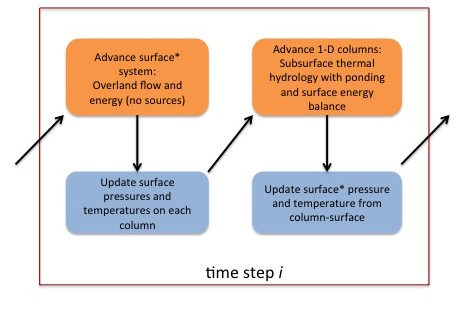
\includegraphics[height = 6.5cm, width=11cm]{figures/Figure5-new.jpg}
\caption{Schematic of the loosely coupled scheme for our mixed-dimensional model. Orange represents advancement of PKs in time; blue shows intermediate steps for initialization of PKs within a single time step.}
\label{coupling-schematic}
\end{figure}


\subsection{ATS Refactoring Strategy}
The ATS was significantly refactored to accommodate the above customized scheme.
Arcos's state object stores a dynamic, runtime-determined set of simulation data.
Each data is identified by a unique key, e.g. ``ponded\_depth'', and a set of metadata including domain of applicability, mesh entity, number of degrees of freedom, etc.
In order for each PK to be instantiated multiple times, that PK's data was altered to enforce uniqueness of its keys by prefixing a domain identifier such as ``column\_0\_surface-ponded\_depth''.
This refactoring allows multiple instances of any given PK, each attached to a different mesh representing a subdomain of the primary mesh.

Furthermore, Amanzi-ATS relies on a meshing infrastructure, MSTK, \cite{garimella-2014-mstk}  which can generate meshes as subdomains or subsets of existing meshes.
This framework was extended to allow column meshes to be generated from an existing three-dimensional mesh.
In this workflow, a surface mesh consisting of the surface polygons are extruded vertically, following pre-determined soil horizon structure, to create a 3D mesh.
By insisting that the extrusion process works only in the vertical, well-defined columns then exist in the the three-dimensional mesh.
At run-time, columns can then be identified, and extracted to form a one-dimensional mesh.
This mesh is altered to ensure it is a one-dimensional submanifold of three-dimensional space, i.e. each cell has two faces, and all face-normals are $\pm \hat{z}$.
Once this is done, Amanzi-ATS's existing operators can work on this mesh without changes.
Furthermore, this mesh follows polygonal ground, and therefore consists of stacked polygonal-prisms.
Few mesh capabilities support this fully-unstructured mesh type; a Silo\cite{silo} capability was added to to Amanzi-ATS's existing output options to enable visualization of the resulting solution.

Each of these refactors was accomplished in reasonable time thanks to a close adherance to computational software best-practices.
A series of unit and regression tests were added for each new capability, and the existing regression tests were updated with the domain prefixes.
Version control enabled close collaboration on this process across multiple developers, and project-management Kanban tools were used to ensure each developer in the workflow knew the needs of the client code component.
These best-practices, along with the use of libraries such as Silo, MSTK, and Arcos, greatly improved the efficiency of what otherwise would have been a significant development effort.

\section{Results and Discussions}\label{numerical-tests}

In this section, we present numerical results that highlights the accuracy and efficiency of our modeling technique. At the development stage, several numerical experiments were performed to verify the physical behavior of the refactored modules (PKs) of the ATS, code verification details are presented in~\ref{code-verification}. The spinup process (i.e., model's initialization) has been described in detail in~\cite{spainter2016integrated}. 


\subsection {Numerical Results -- A Comparative Study} 
To demonstrate the accuracy of our modeling technique, we compare numerical results of the mixed-dimensional model against a fully coupled three-dimensional simulations that act as a benchmark for our simulations. The domain under consideration has surface elevation varying between 4.14-4.62 m, is 40 m deep, and enclosed by a rectangle in the horizontal plane 173 $\times$ 160 m$^2$; see Fig.~\ref{surf-location}. This domain is a part of the low-gradient polygonal tundra in Barrow, Alaska and consist of 75 ice wedge polygons. As highlighted in Fig.~\ref{surf-location}, we select five spots (based on different elevations) to perform a location-based comparison of the numerical results of the two schemes. 
\begin{figure}[!htpb]
\centering
%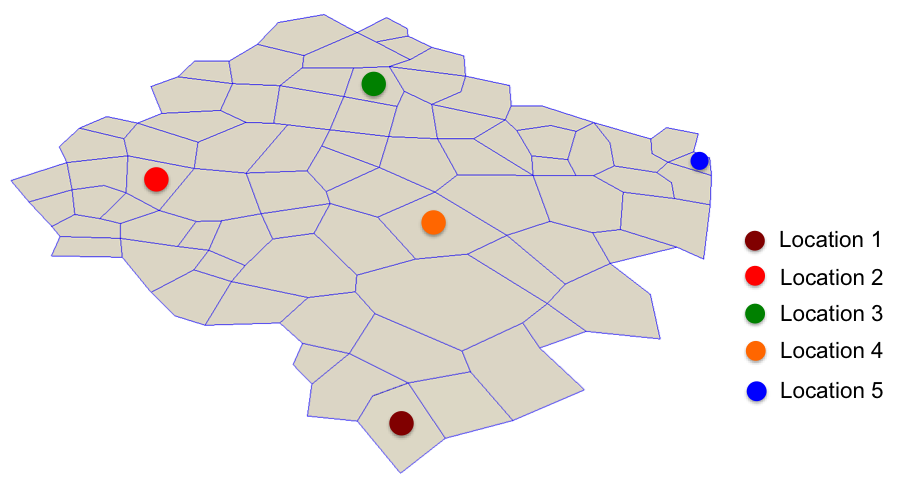
\includegraphics[height = 5.5cm, width=9cm]{figures/surface-locations.png}
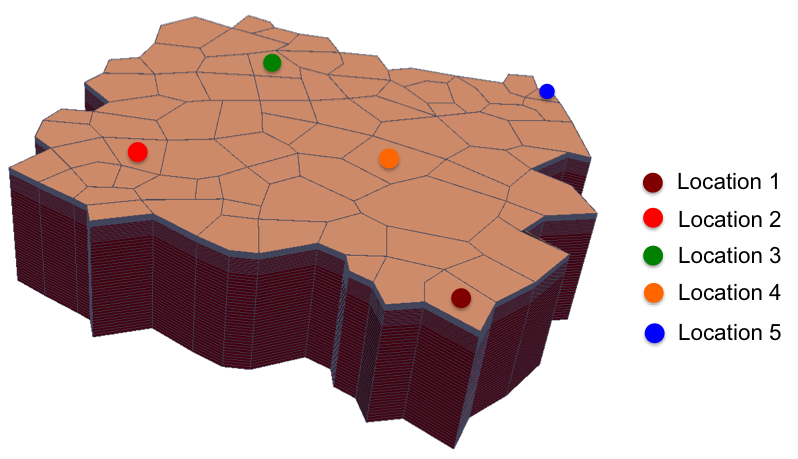
\includegraphics[height = 6.5cm, width=11cm]{figures/lobster75-3d.png}
\caption{An illustration of the five spatial locations on 75 polygons cluster for location-based comparison of the two schemes. Location 1: Outlet. Location 2: High elevated spot. Location 3-4: Intermediate elevation spots. Location 5: Lowest elevation spot.}
\label{surf-location}
\end{figure}

In addition to evaluating the quality of our mixed-dimensional approach for the Barrow tundra, we also want to understand when it will give inaccurate results. Because our modeling strategy is based on a loosely coupled scheme and neglects subsurface lateral flow between ice wedge polygons, it should eventually become inaccurate if the topographic relief is sufficiently large. To identify the range of applicability, we consider three variants of the surface topography.  We use the following equation to exaggerate the surface topography,
\begin{equation}\label{formula-exagg}
\bar{Z} =  \alpha (Z - \mu) + \mu.
\end{equation}
Here $\bar{Z}$ is the exaggerated elevation, $Z$ is the original elevation with mean $\mu$, and $\alpha$ is the exaggeration parameter. Equation~(\ref{formula-exagg})  preserves the mean while the standard deviation depends on the value of $\alpha$ and is given in meters by $0.14 \alpha$. The coefficient in front of $\alpha$ is the standard deviation of the original elevation $Z$ -- in our case $Z$ correspond to the domain shown in Fig.~\ref{surf-location}. Our three variants correspond to $\alpha=1,3,$ and $5$. The value $\alpha=1$ corresponds to the original topography. We expect the model to give promising results for simulating low-gradient polygonal tundra, and believe that the values of $\alpha$ we choose provide sufficient variation across a domain of 100s of meter. 
Our numerical experiments confirm a high agreement between the results of the mixed-dimensional model and the 3D model at all selected location for all three $\alpha$ values. Figs.~\ref{ss-sat-comp} and~\ref{ss-temp-comp} compare the subsurface water saturations and temperatures, respectively, at locations 1 and 5 and for $\alpha=1$. The accuracy of our results for the Barrow topography ($\alpha=1$) is evident. The surface ponded depths and temperatures obtained with the two models are depicted in Fig.~\ref{surf-pd-comp} and~\ref{surf-temp-comp}, respectively. As expect, our results fit the 3D model's results very well. We see the same level of agreement at the other locations as well, but we are not showing them here.
%The root mean square difference in the subsurface water saturations of the two models of study-I, II, and III are shown in Fig.~\ref{error-plots}.
In Fig.~\ref{thaw-depth} we plot the mean annual thaw depth at five locations for the three variants, $\alpha =1, 3,$ and $5$. We use the annual mean of the thaw depth rather than the maximum thaw depth (i.e. the active layer thickness) because the mean annual thaw depth depends on both the duration of thaw and maximum thaw depth. Thus it is a direct measure of soil available for decomposition, averaged over the year. 
Not surprisingly, as the value of $\alpha$ increases the mean annual thaw depth deviates from the results of the 3D model to some extent, but we still see the results of the mixed-dimensional model agree well with to the corresponding benchmark solution. The consistency of our numerical results with the fully coupled 3D simulations confirm the appropriateness of this approximated scheme. 






 \begin{figure}[!htpb]
\centering
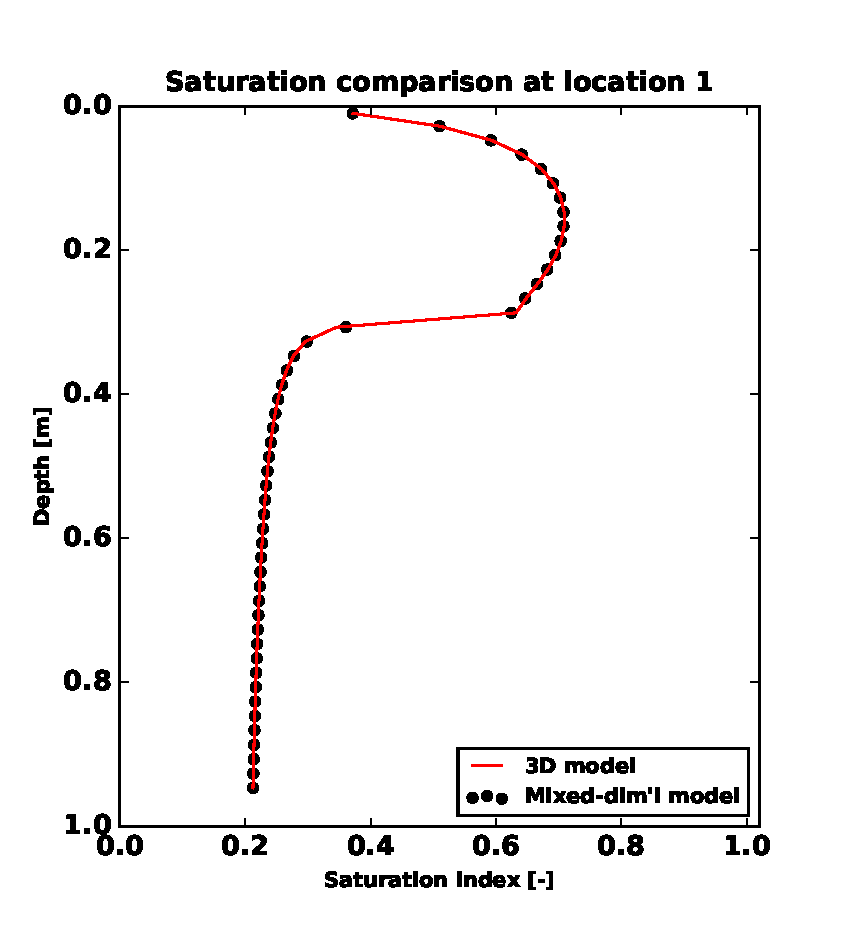
\includegraphics[height = 7.5cm, width=6cm]{figures/comparison/regular/ss-sat/comp-sat-loc1-cycle0020.eps}
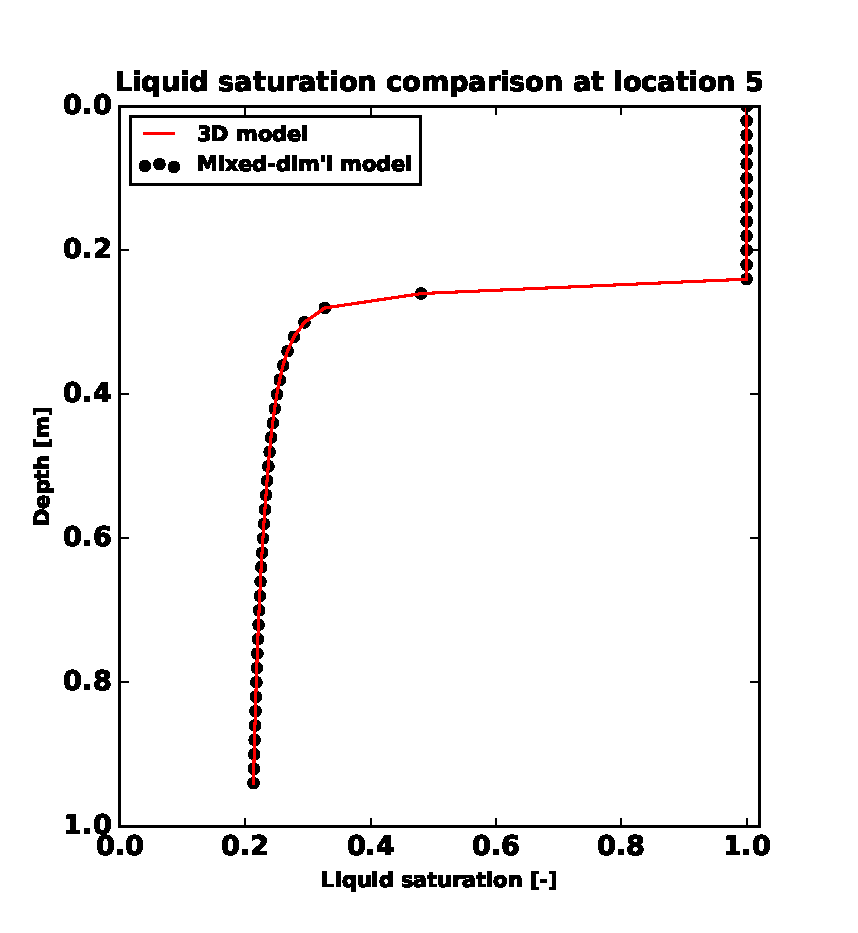
\includegraphics[height = 7.5cm, width=6cm]{figures/comparison/regular/ss-sat/comp-sat-loc5-cycle0020.eps}
\caption{Comparison of the subsurface water saturation at locations 1 and 5 during the summer.}
\label{ss-sat-comp}
\end{figure}


\begin{figure}[!htpb]
\centering
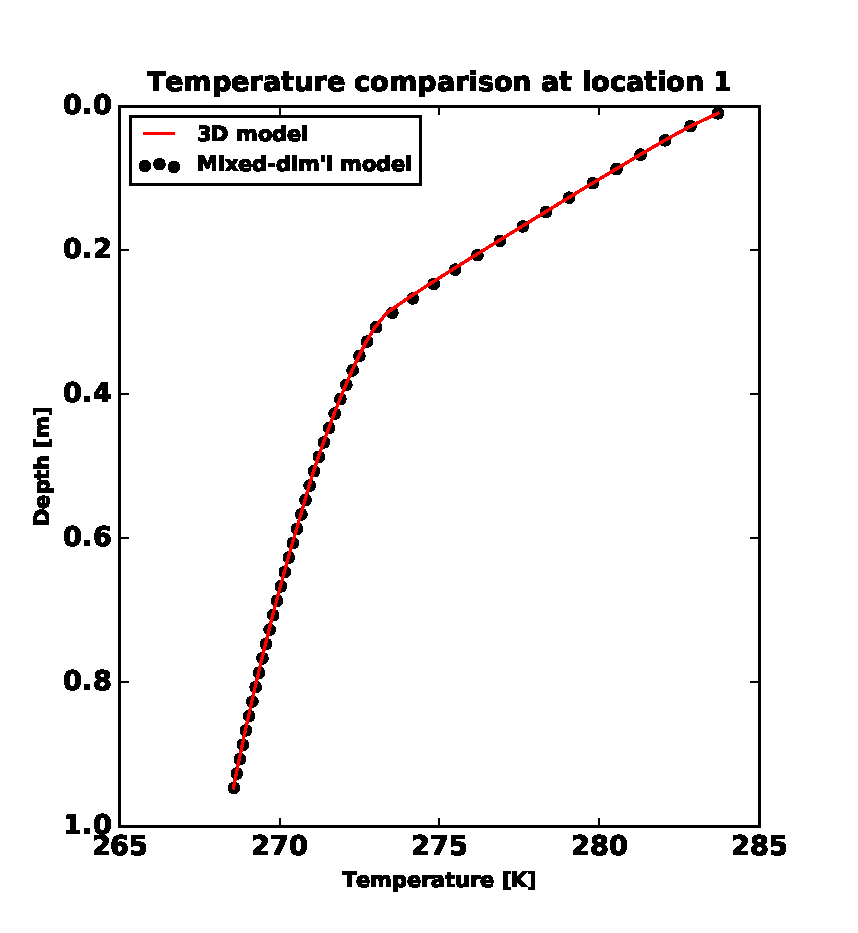
\includegraphics[height = 7.5cm, width=6cm]{figures/comparison/regular/ss-temp/comp-temp-loc1-cycle0020.eps}
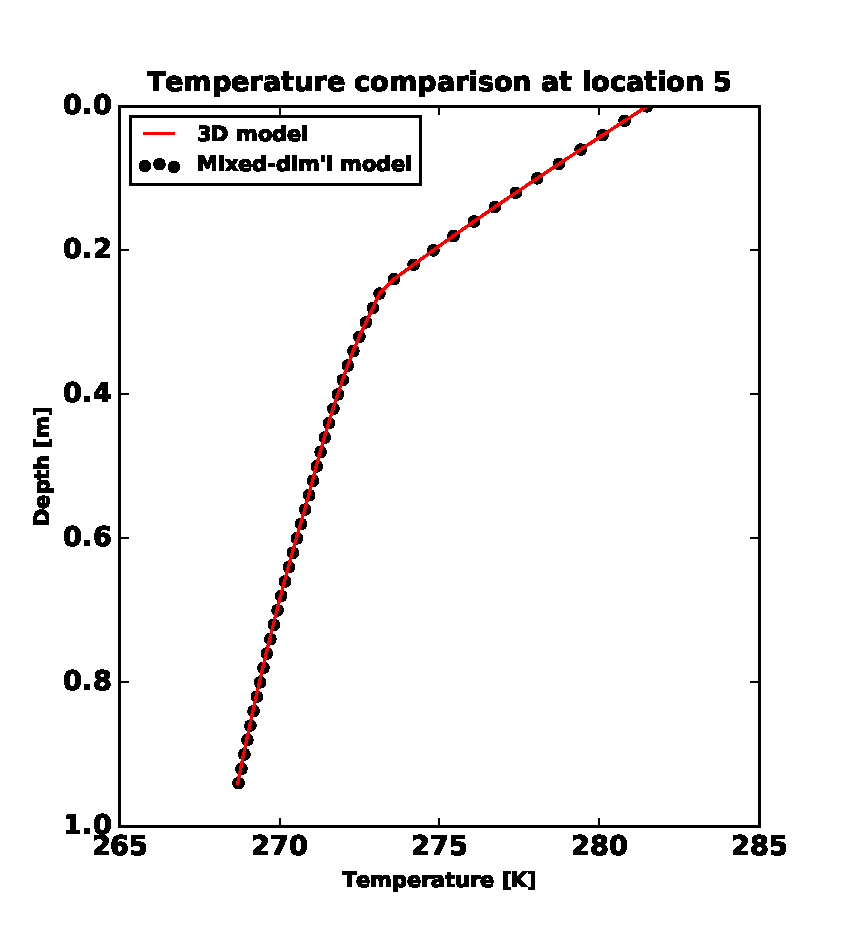
\includegraphics[height = 7.5cm, width=6cm]{figures/comparison/regular/ss-temp/comp-temp-loc5-cycle0020.eps}
\caption{Comparison of subsurface temperature at locations 1 and 5 during the summer.}
\label{ss-temp-comp}
\end{figure}

\begin{figure}[!htpb]
\centering
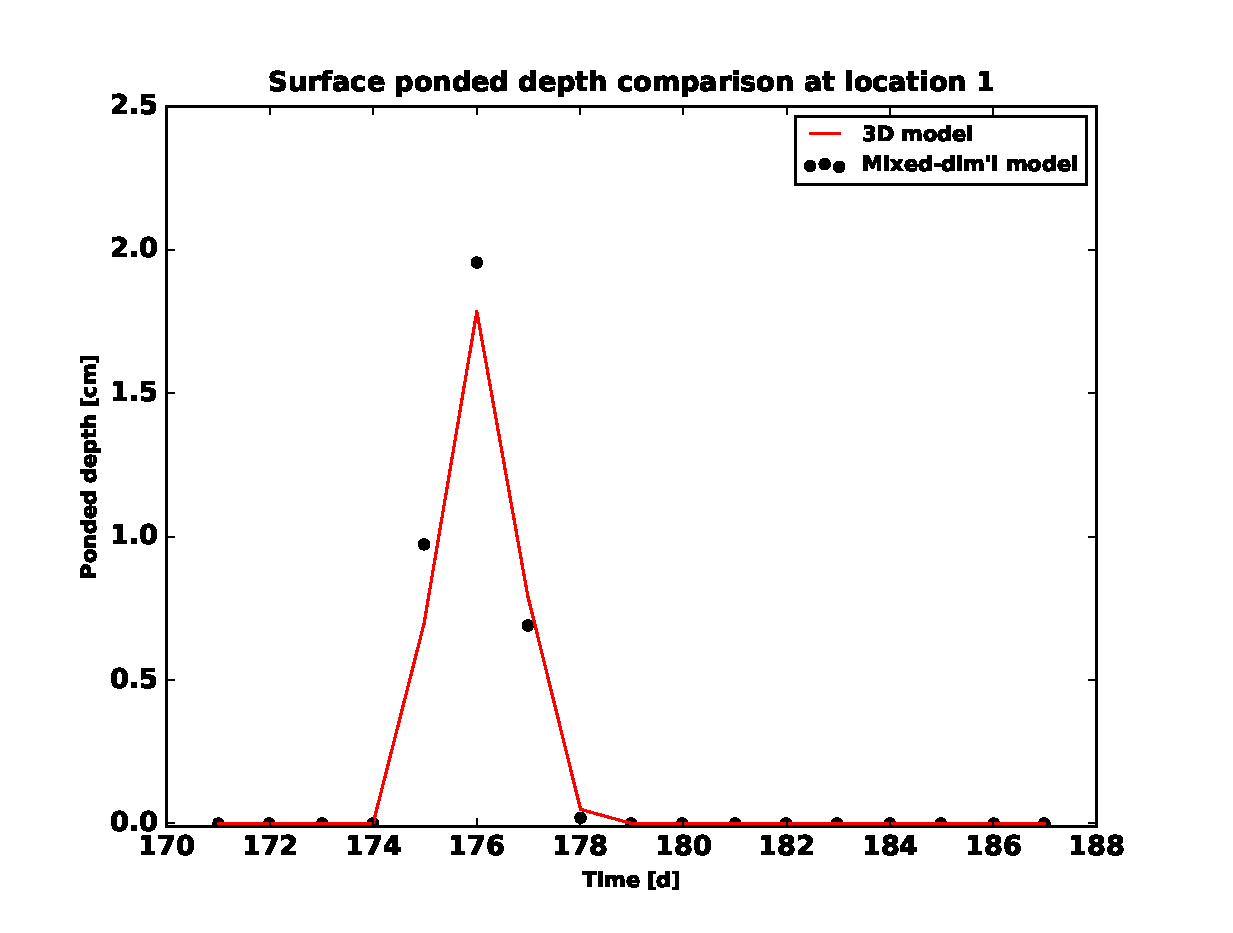
\includegraphics[height = 7.5cm, width=6.cm]{figures/comparison/regular/ponded-depth/comp-pd-location1.eps}
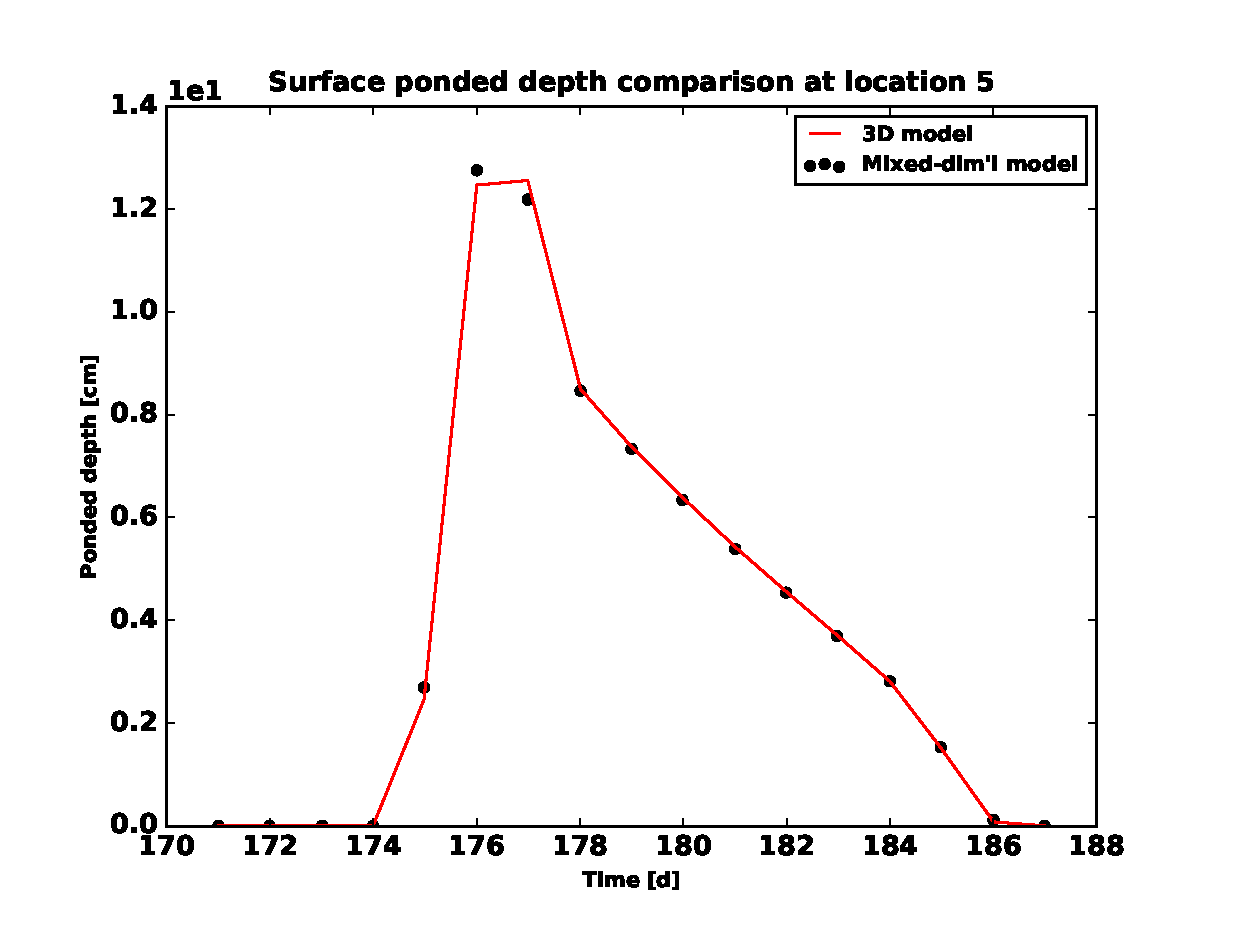
\includegraphics[height = 7.5cm, width=6.cm]{figures/comparison/regular/ponded-depth/comp-pd-location5.eps}
\caption{An illustration of the surface ponded depths of the two schemes at locations 1 and 5 when the snow melt starts.}
\label{surf-pd-comp}
\end{figure}

\begin{figure}[!htpb]
\centering
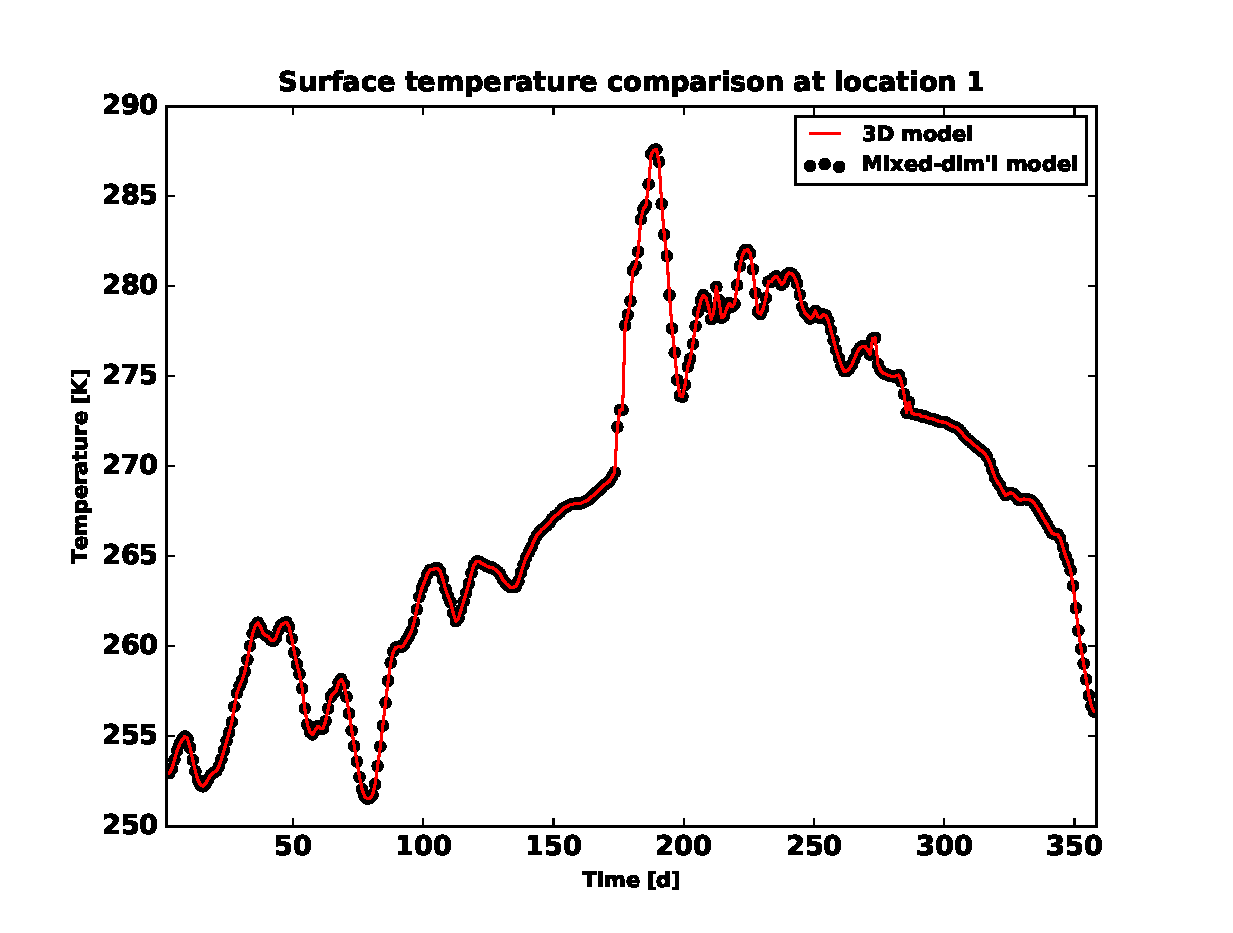
\includegraphics[height = 7.5cm, width=11.cm]{figures/comparison/regular/surf-temp/comp-temp-location1.eps} \\
%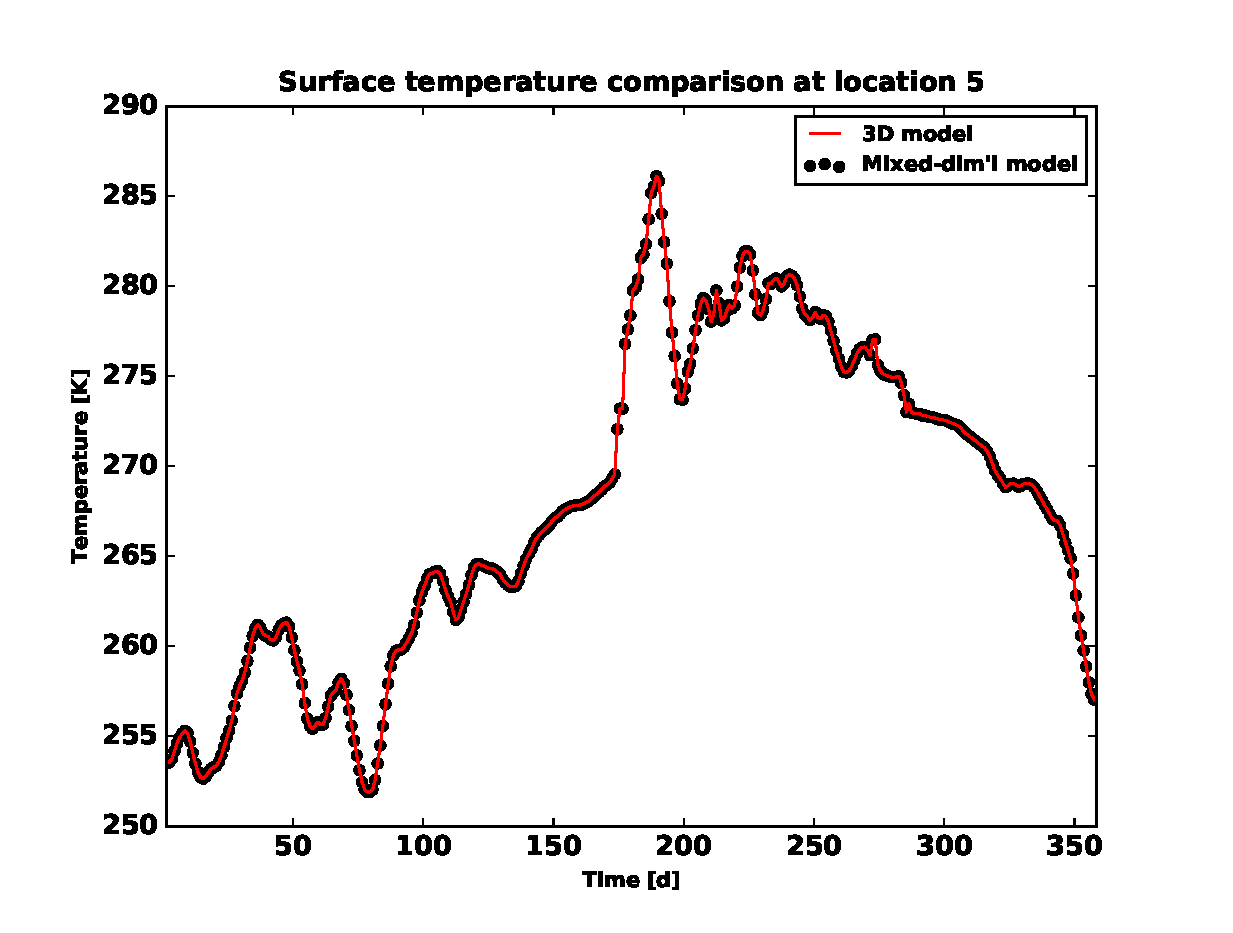
\includegraphics[height = 5.9cm, width=11.cm]{figures/comparison/regular/surf-temp/comp-temp-location5.eps}
%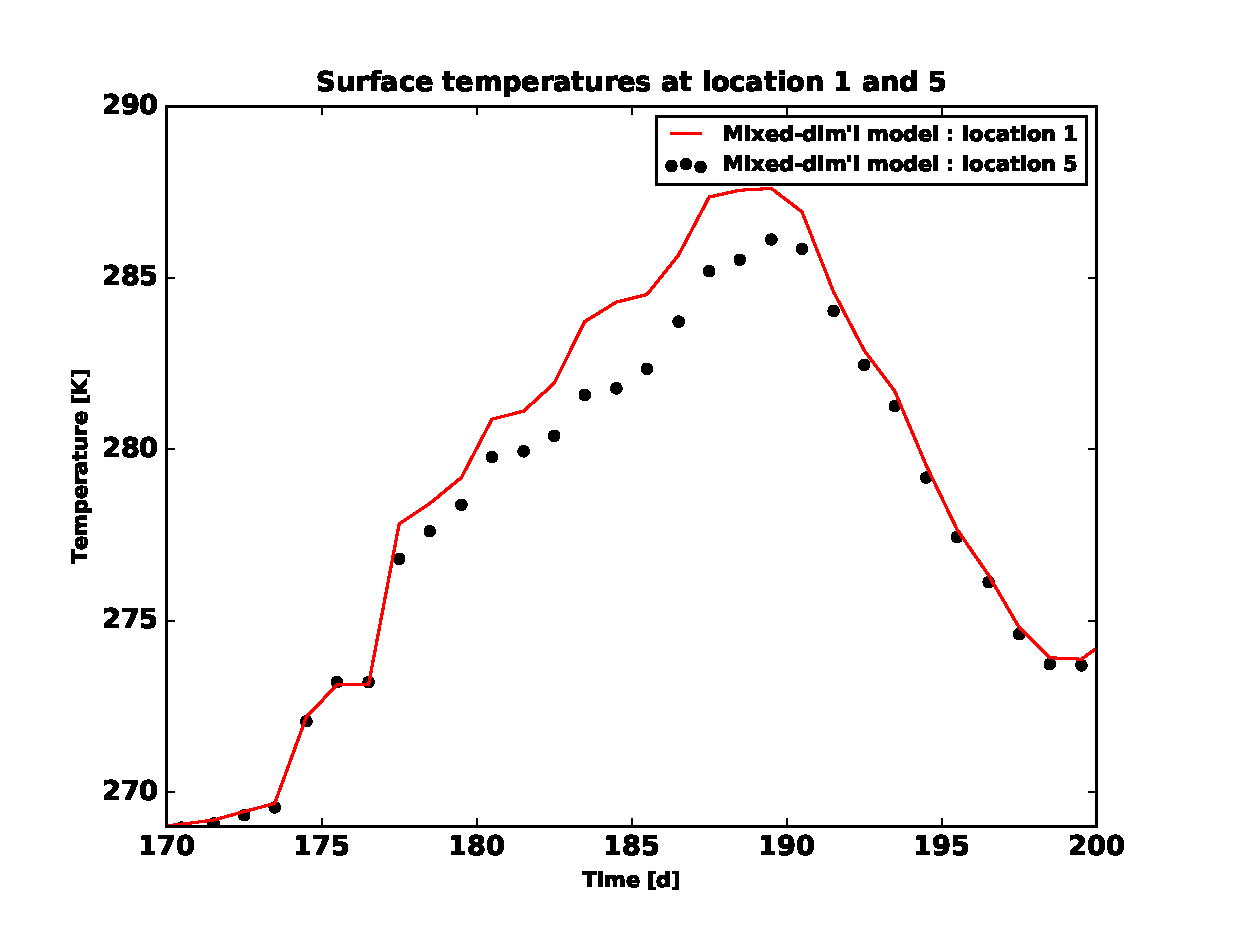
\includegraphics[height = 5.9cm, width=11.cm]{figures/comparison/regular/surf-temp/comp-temp-location1-5.eps}
\caption{An illustration of the surface temperature of the two schemes at location 1 for the entire year. %The bottom plot highlights the difference between the temperatures at location 1 and 5, though they appear quite similar in the top two plots.
}
\label{surf-temp-comp}
\end{figure}

%\begin{comment}
%\begin{figure}[!htpb]
%\centering
%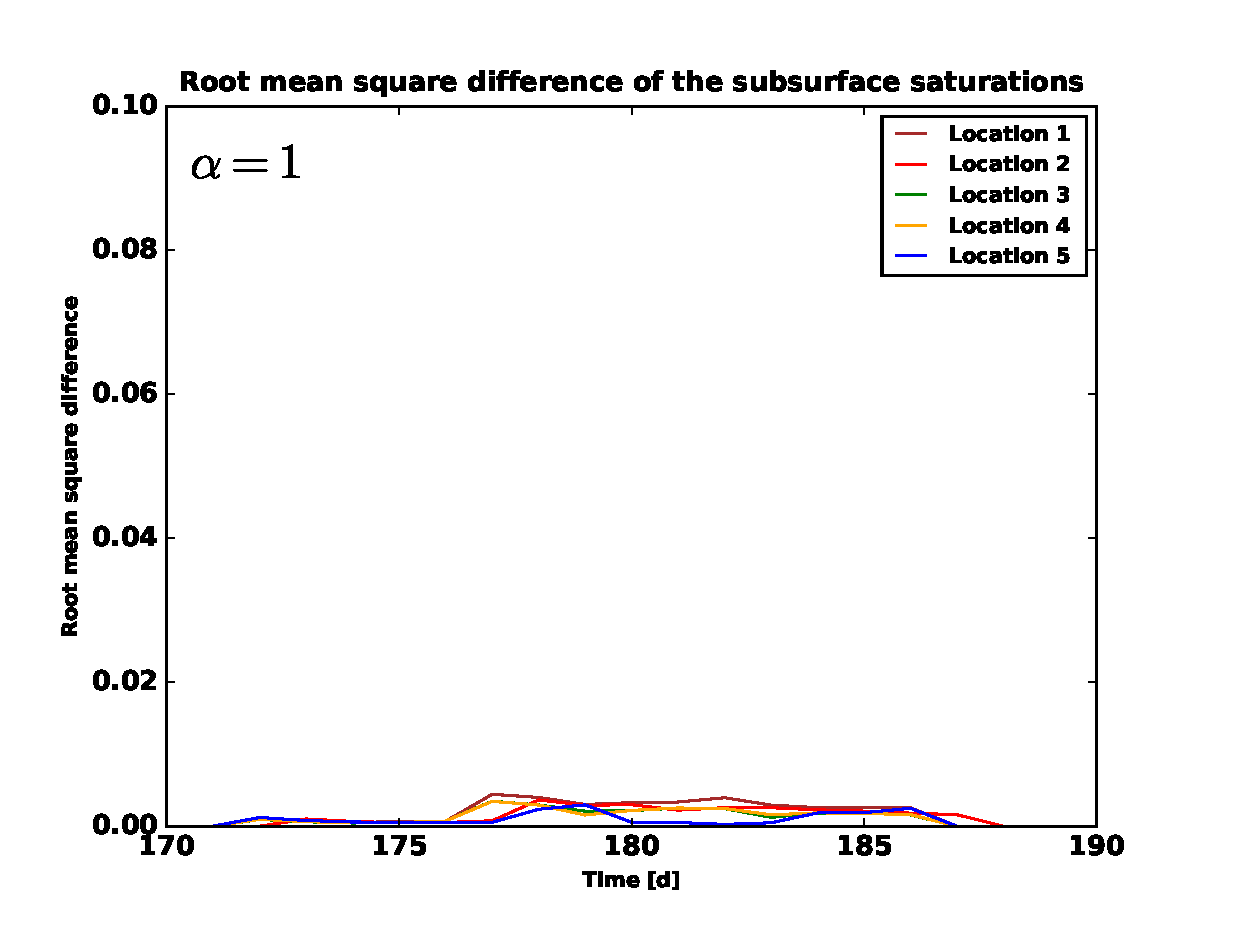
\includegraphics[height = 6.cm, width=10.cm]{figures/comparison/regular/error.eps}
%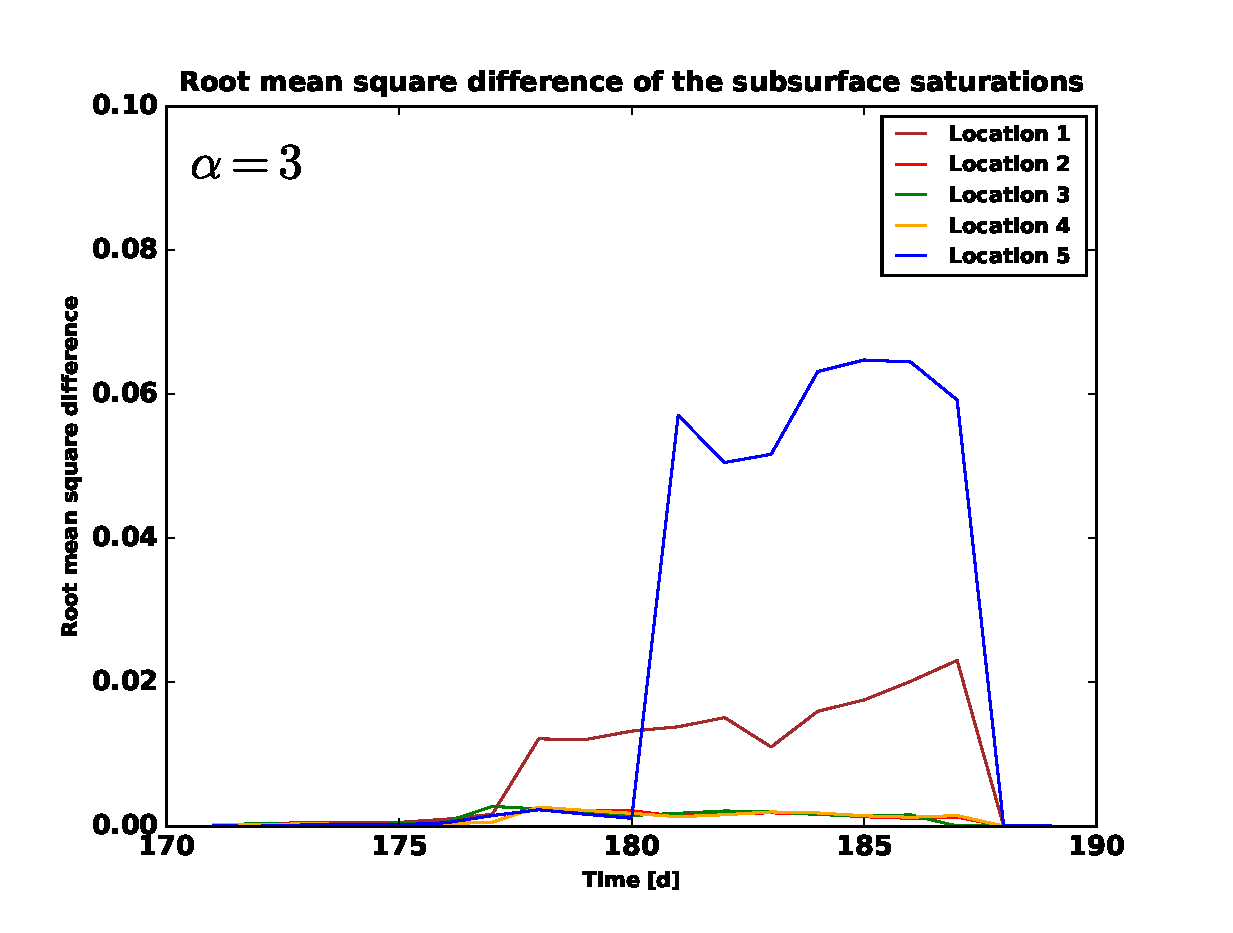
\includegraphics[height = 6.cm, width=10.cm]{figures/comparison/dist/Elev-grad1.5m/error.eps}
%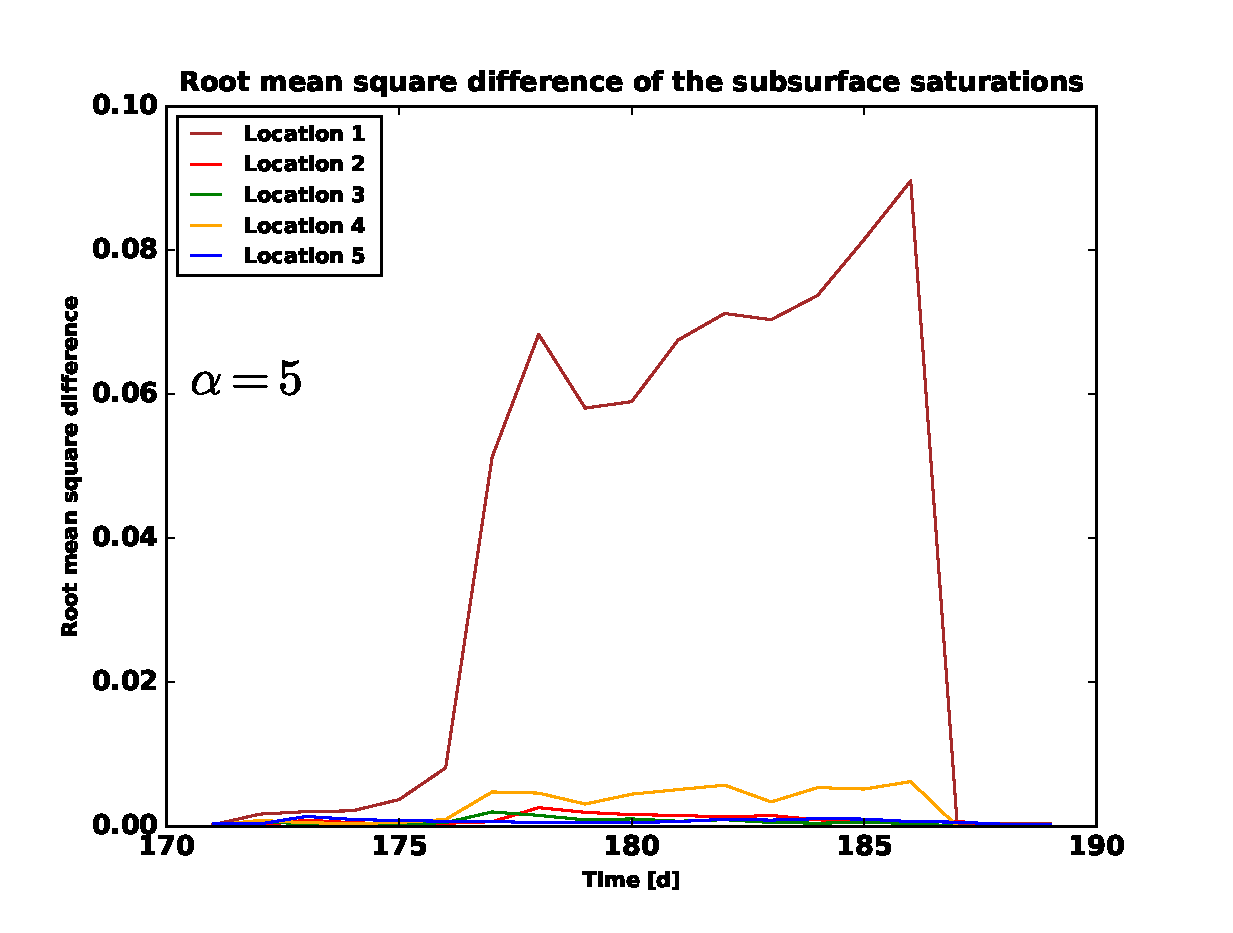
\includegraphics[height = 6.cm, width=10.cm]{figures/comparison/dist/Elev-grad2.5m/error.eps}
%\caption{The root mean square difference of the subsurface water saturation at the selected locations of the three studies.}
%\label{error-plots}
%\end{figure}
%\end{comment}

\begin{figure}[!htpb]
\centering
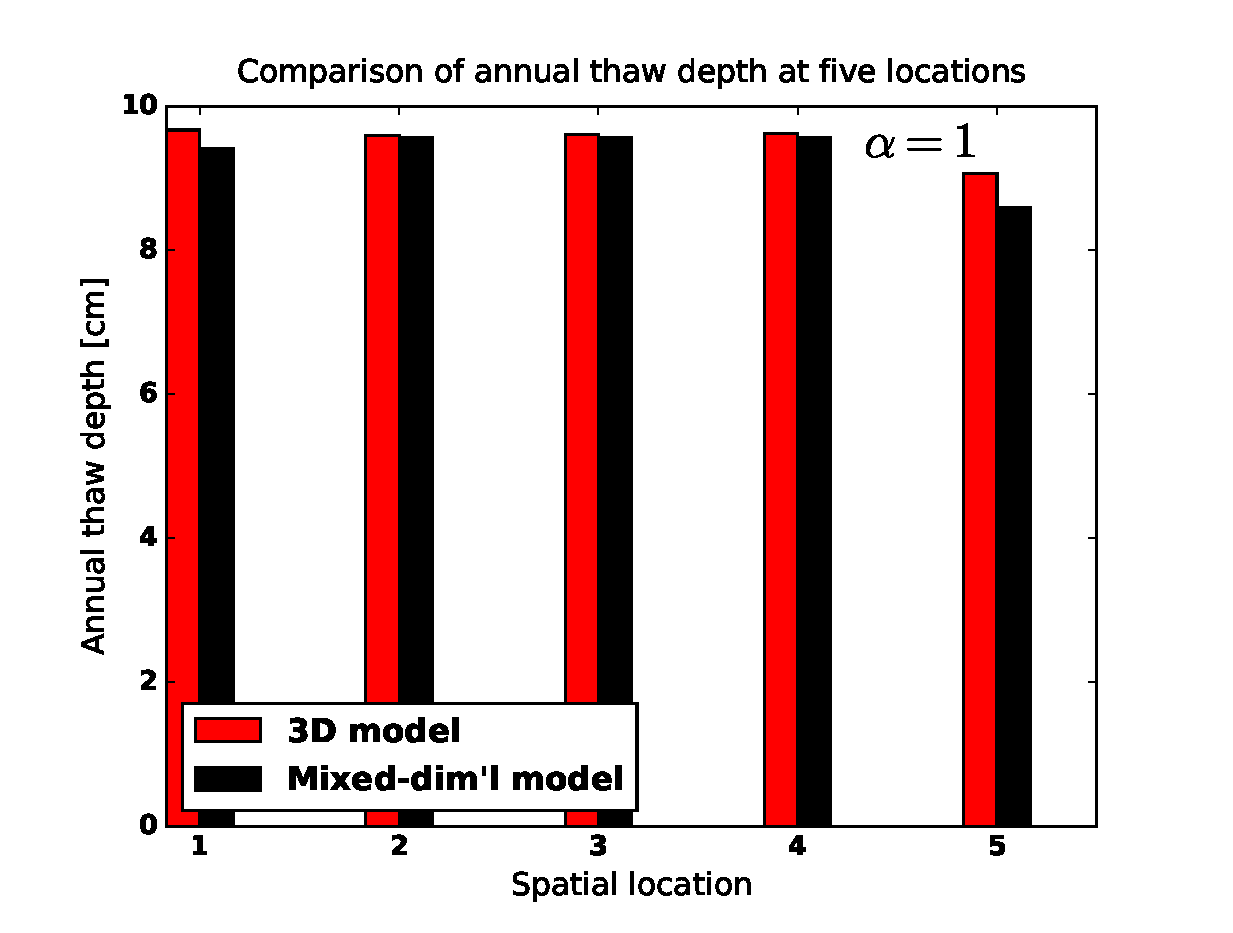
\includegraphics[height = 6.cm, width=10.cm]{figures/comparison/annual-thaw-depth/annual_depth-1.eps}
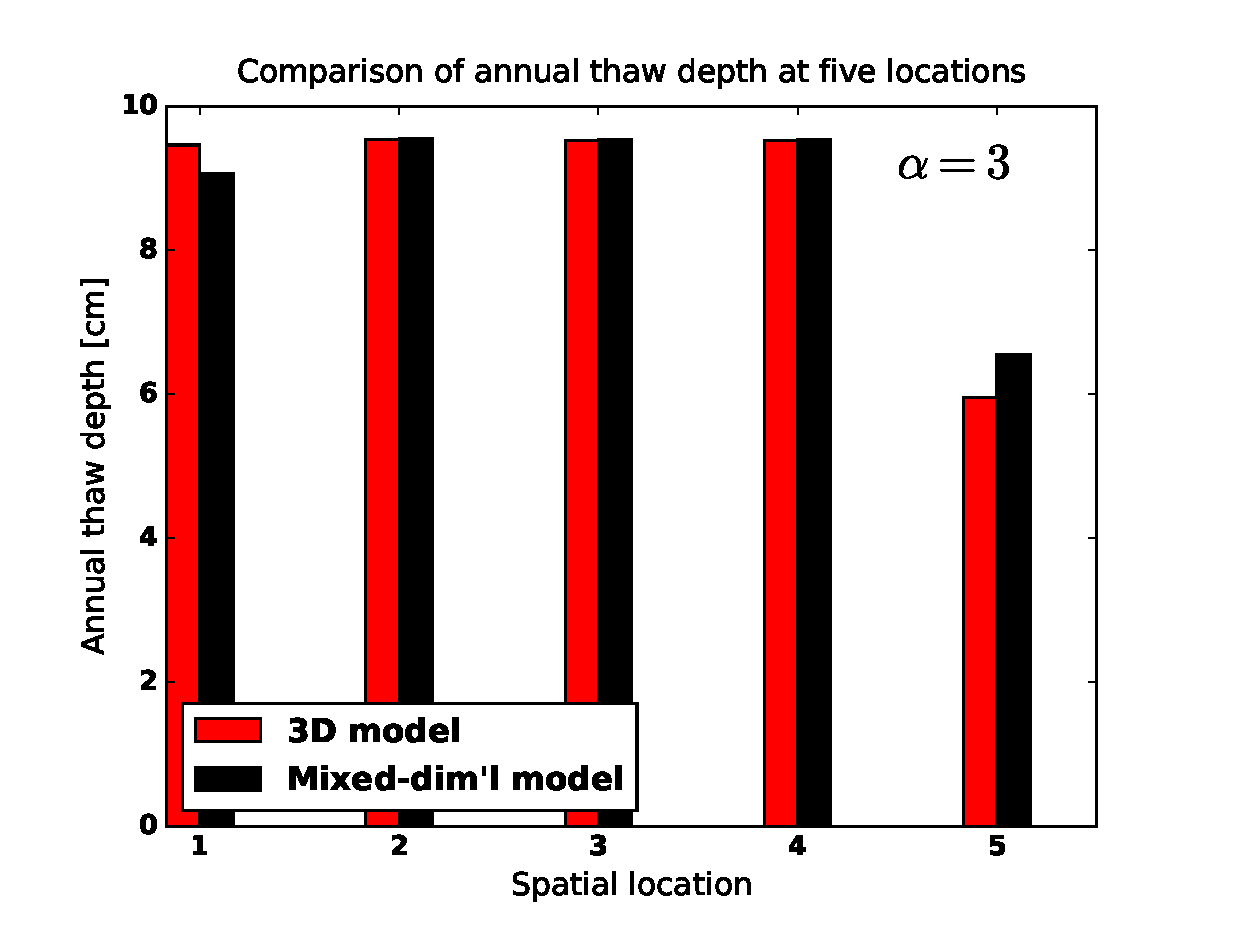
\includegraphics[height = 6.cm, width=10.cm]{figures/comparison/annual-thaw-depth/annual_depth-3.eps}
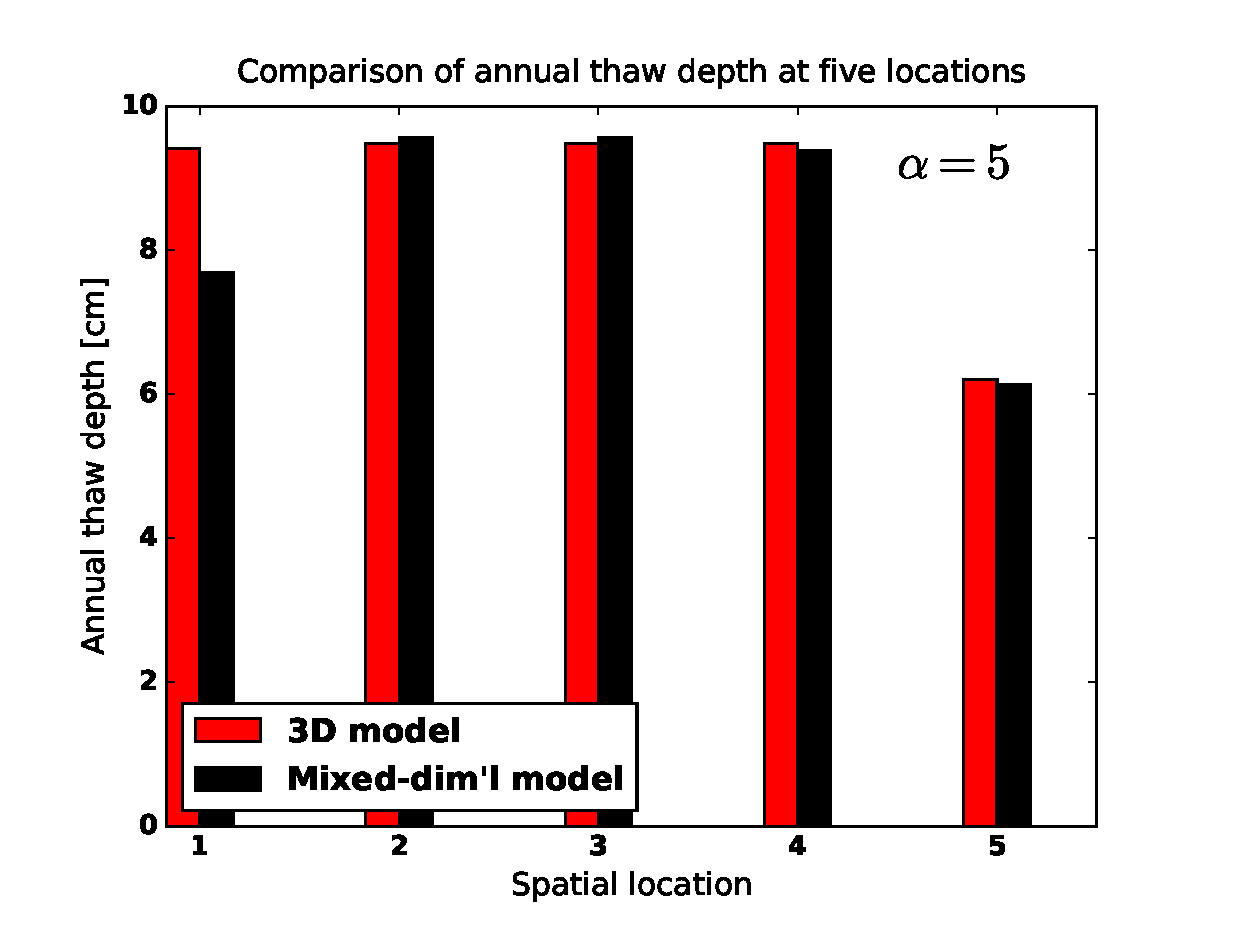
\includegraphics[height = 6.cm, width=10.cm]{figures/comparison/annual-thaw-depth/annual_depth-5.eps}
\caption{A comparison of the annual thaw depth at the selected locations of the three studies.}
\label{thaw-depth}
\end{figure}


\begin{figure}[!htpb]
\centering
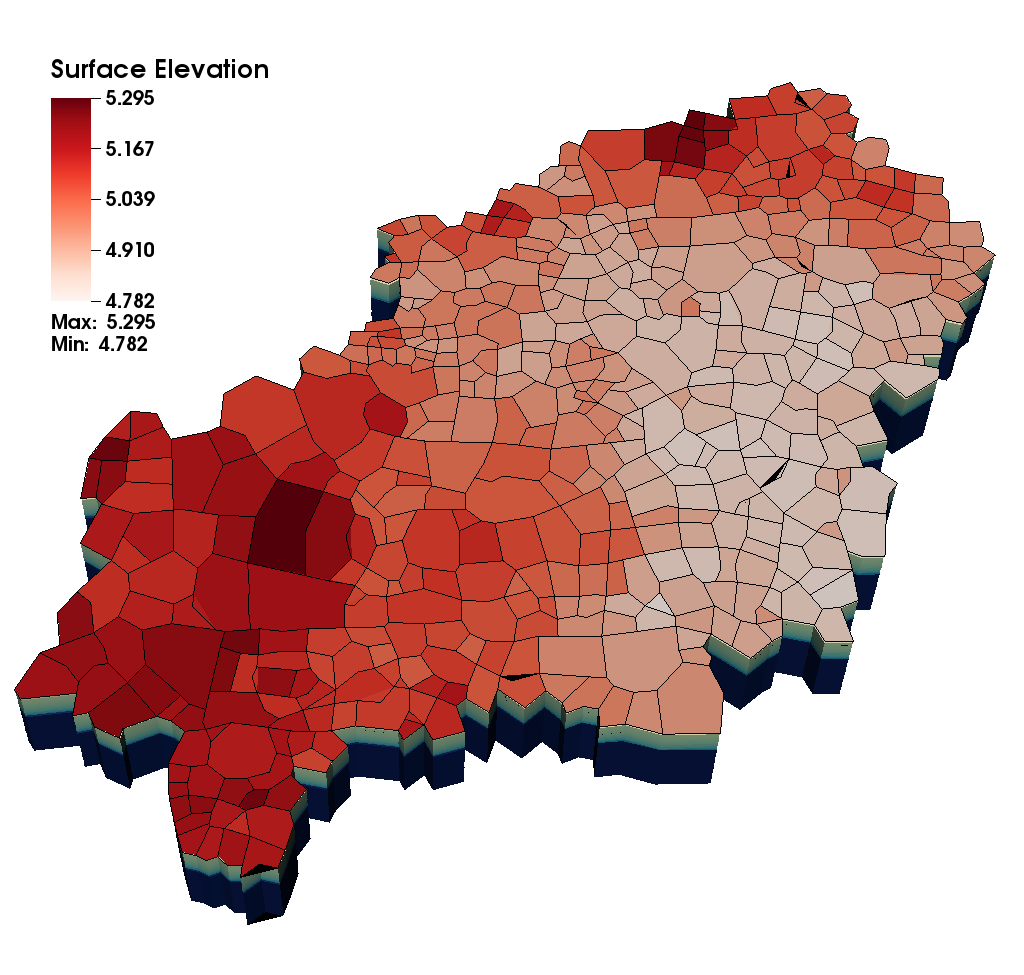
\includegraphics[height = 8.5cm, width=11cm]{figures/barrow-watershed-image-3.png}
\caption{A watershed at Barrow, Alaska.}
\label{barrow-468}
\end{figure}
 
 \begin{figure}[!htpb]
\centering
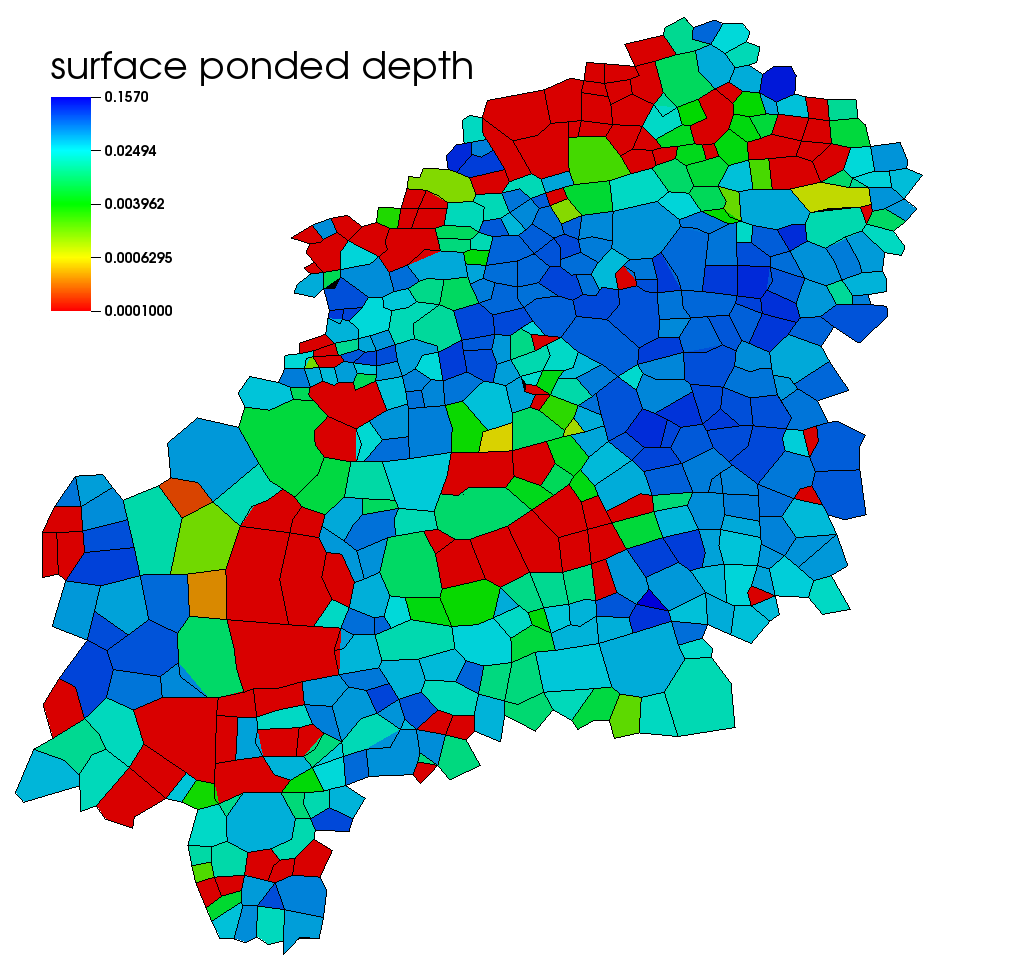
\includegraphics[height = 7.5cm, width=12cm]{figures/surface-ponded-depth3-time13-4507.png} \\
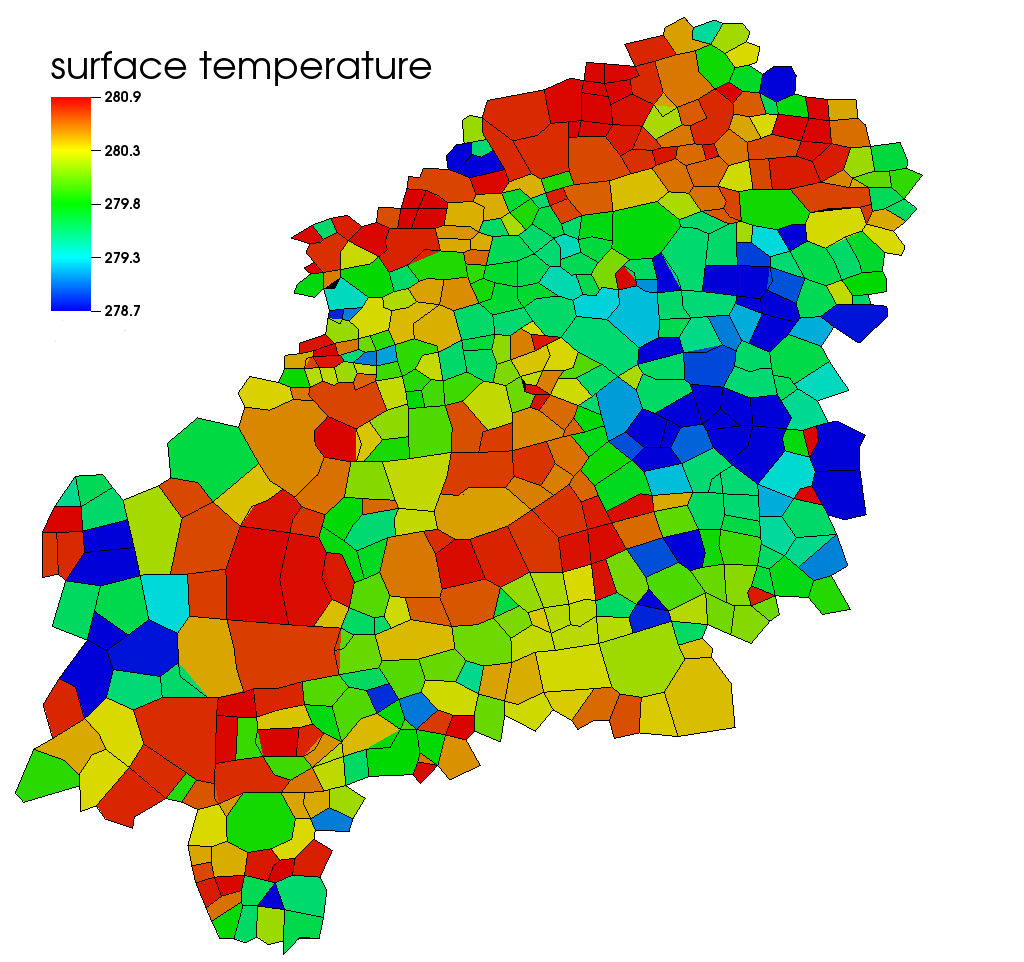
\includegraphics[height = 7.5cm, width=12cm]{figures/surface-temperature3-time13-4644.png}
\caption{Simulation results of the mixed-dimensional model. Showing the surface ponded depth and temperature during the snowmelt of 2012.}
\label{barrow-pd-temp}
\end{figure}

%\todo{should we provide a Table describing Parameters used in the simulations}

\subsection{Speedup Study}
We discuss speedup and parallel efficiency for two spatial domains, one with 75 polygons as depicted in Fig.~\ref{surf-location} and a larger one consisting of 468 ice-wedge polygons, as shown in Fig~\ref{barrow-468}. The surface ponded depth and temperature during the snowmelt in 2012 are presented in Fig.~\ref{barrow-pd-temp} for the 468 polygon domain. Fully coupled 3D simulations at such a scale are computationally very expensive.

We highlight two aspects of the efficiency of this modeling approach: (i) how the simulation time decreases in comparison with three-dimensional simulations, and (ii) how efficiently it scales with number of processes. 

Fig.~\ref{3d-lcs-speed} compares the computational time of the multidimensional strategy versus the three-dimensional solution for the domain consisting of 75 columns. 
It can be seen that for a fixed number of processors, the computational time decreases by a factor of about four with the multidimensional technique. This is a huge computational advantage without sacrificing numerical accuracy. 

We show parallel strong scaling for the aforementioned domains in Fig.~\ref{lcs-speed}. Speedup of the smaller domain is significantly less than the linear ideal; this is caused by communication overhead in the surface* system. Without consideration of the surface* system, the problem is perfectly parallel. To minimize communication between the surface* system and the column systems, the surface* mesh is partitioned so that a column and the coincident mesh cells on the surface* system reside on the same processor. If there are too few columns per processor, the interprocessor communication for the surface* system becomes the limiting factor despite the lower computational burden for the surface* system compared with the columns. 
As expected, the scaling is better for a larger domain. Scaling is close to linear up to about 16 cores, which corresponds to about 30 columns per core. 

\begin{figure}[!htpb]
\centering
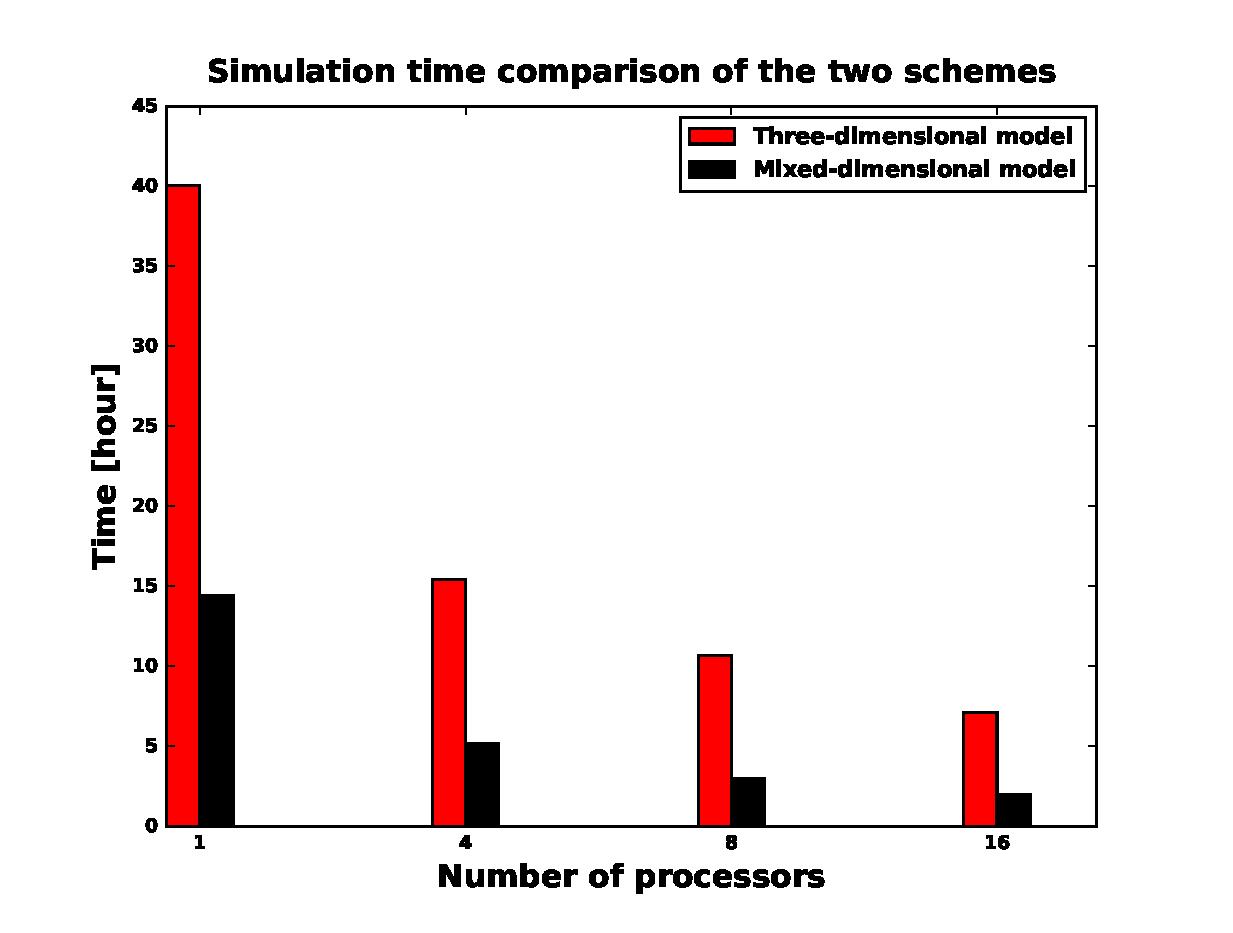
\includegraphics[height = 6.5cm, width=10cm]{figures/compare3d-lcs-speed.eps}
\caption{A comparison of the computational time taken by the mixed-dimensional and 3D models.}
\label{3d-lcs-speed}
\end{figure}


\begin{figure}[!htpb]
\centering
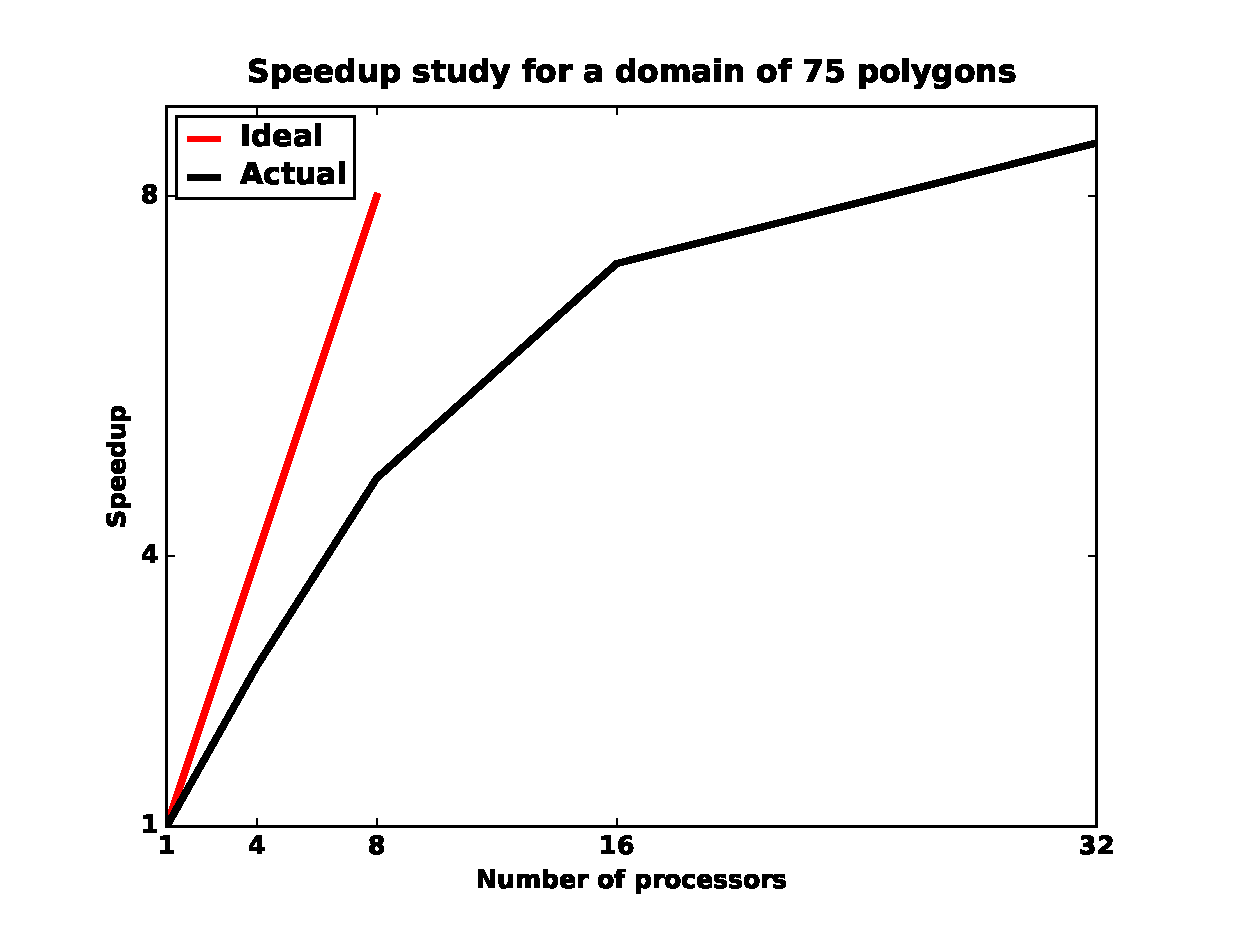
\includegraphics[height = 6.5cm, width=10cm]{figures/speedup-lcs-lobster.eps}
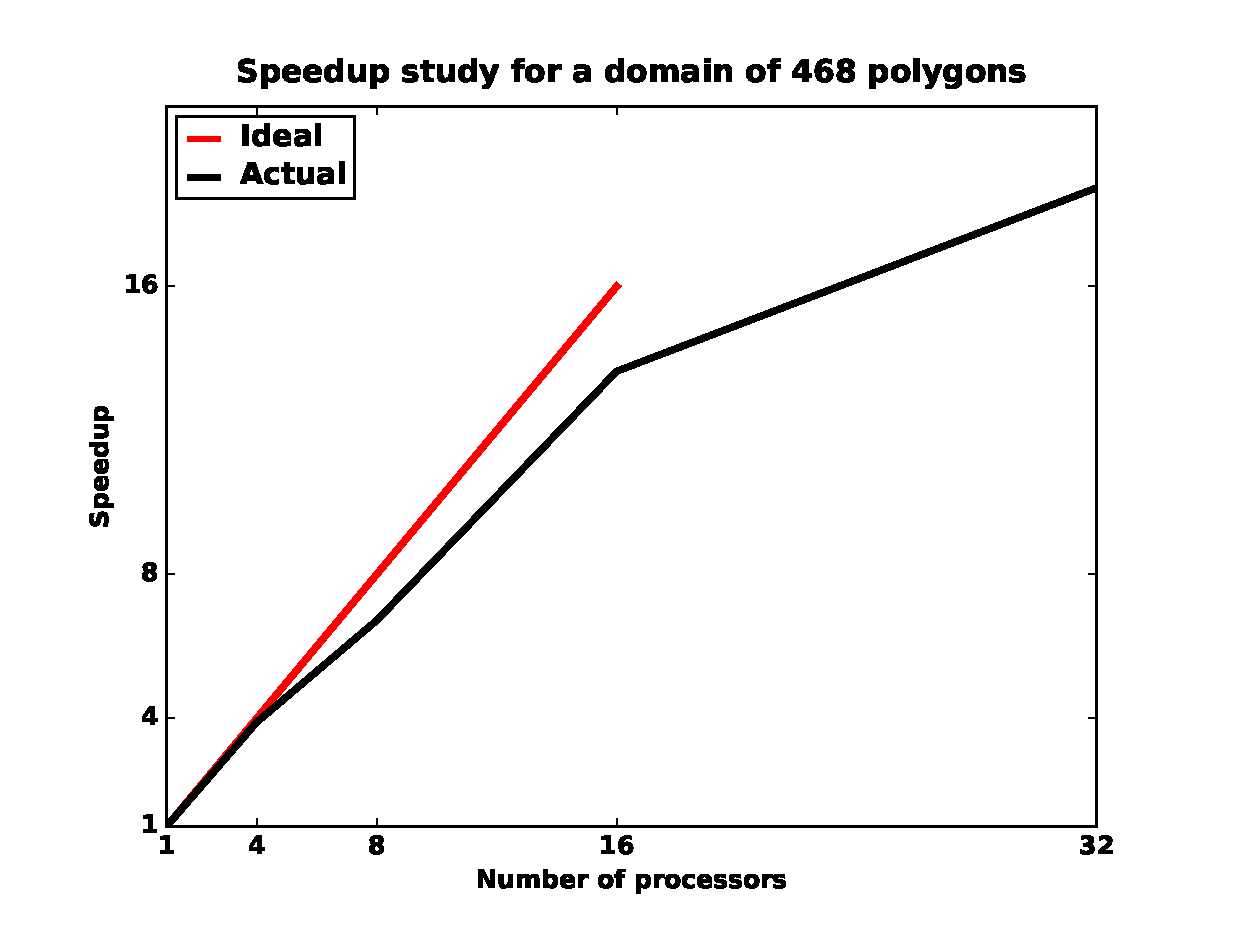
\includegraphics[height = 6.5cm, width=10cm]{figures/speedup-lcs-barrow.eps}
\caption{An illustration of the speedup study of a simulation with 75-polygon cluster (top) and 468 polygons barrow watershed (bottom).}
\label{lcs-speed}
\end{figure}


\subsection{Subcycling Process Kernels}
One advantage of sequentially coupling different PKs, as opposed to a fully coupled approach, is that sequential coupling makes subcycling possible. With subcycling, individual PKs take their own time step rather than a global time step. The independently evolving PKs are then synchronized on a larger time step. The idea is to assign a suitable local time-step to each subdomain rather than one single global time-step. It is a very convenient approach for simulating permafrost type regions because a relatively small time step may be required when a cell is going through a phase change. Without subcycling, a timestep failure or small timestep caused by phase change in a single cell results in a small global time step. With subcycling, the effects of that phase transition are limited to a single column.  Our mixed-dimensional modeling approach efficiently allows subcycling PKs because we discretize subsurface as independent columns/subdomains. Thus, the subdomains can advance in time with their preferred time-steps until they hit the synchronized time. Fig.~\ref{subcycle-time-reduciton} displays percentage reduction in the simulation time for the domains consisting of 21, 75, and 468 polygons. With the increase in the number of subsurface columns the computational time decreases, and we see up to 40\% reduction in the computational time in comparison with simulations without subcycling. The choice of the synchronization time is crucial, and requires further optimization, which will be studied in future work.

\begin{figure}[!htpb]
\centering
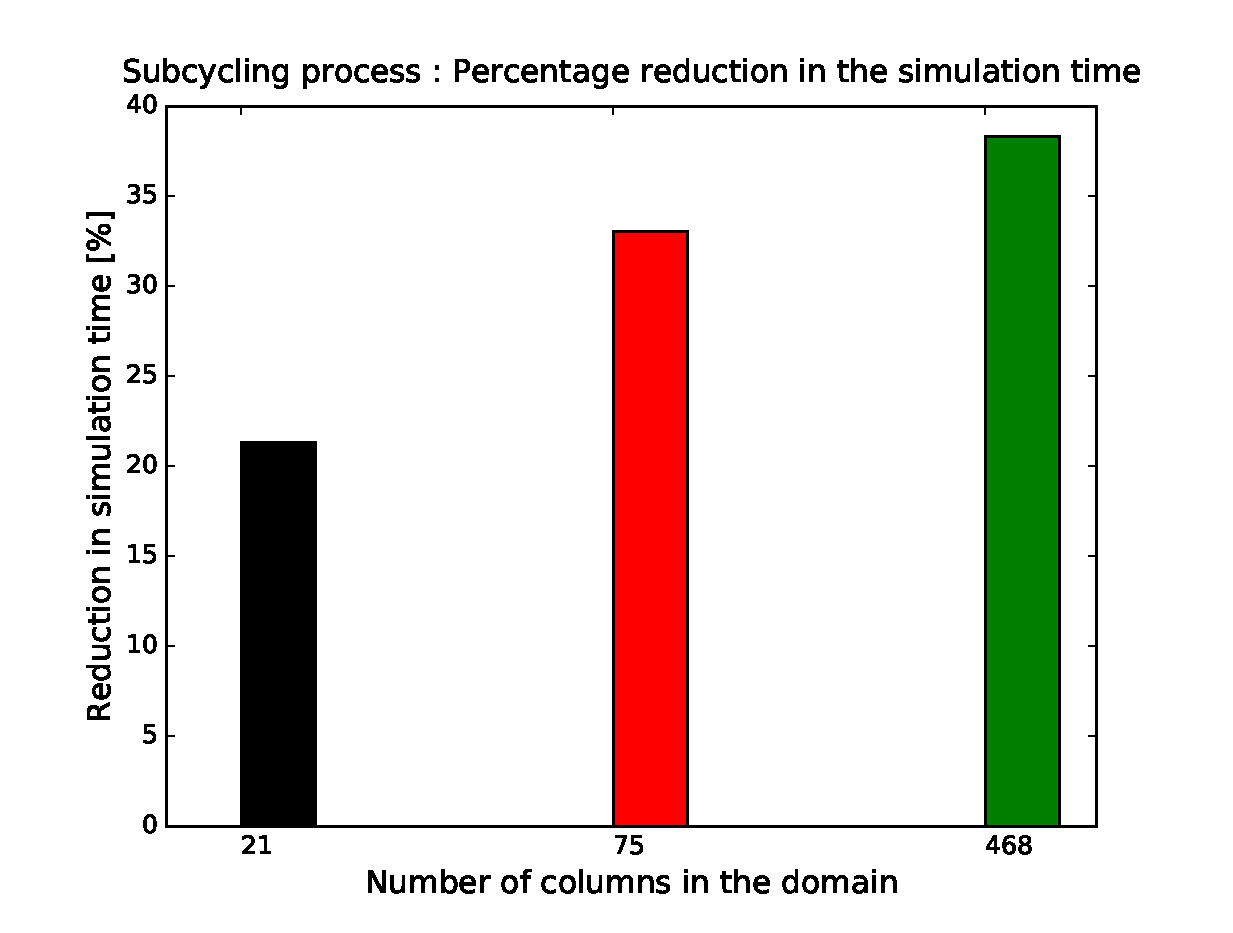
\includegraphics[height = 6.5cm, width=10cm]{figures/subcycle-time-reduciton.eps}
\caption{(Subcycling PKs) Percentage reduction in the computational time for the domains consisting of 21, 75 and 468 polygons. }
\label{subcycle-time-reduciton}
\end{figure}


\section{Conclusions and Future Work}\label{conclusion}

Out intermediate-scale model for integrated surface/subsurface thermal hydrology of low-relief permafrost-affected regions is constructed from two components: a mixed-dimensional spatial structure that is based on discretizing  the subsurface as independent columns that are indirectly coupled through a two-dimensional surface system, and an operator splitting scheme for coupling the column domains to the surface system. The spatial structure was motivated by fine-scale simulations of permafrost regions. This is the first demonstration of advanced representations of freezing soil physics coupled to overland thermal flow and surface energy balance at scales of 100s of meters.

% that explored spatial variations in the thermal conditions among centers, rims, and troughs of ice-wedge polygons during the summer, and mainly equilibrated by lateral heat transport. 
  
%Though this modeling approach has a broader scope but we mainly focus on simulating the thermal hydrology of degrading permafrost (polygonal tundra) near Barrow, Alaska.

%Simulating a fully integrated surface and subsurface thermal hydrology in permafrost-affected regions is both important and challenging. The importance lies in the fact that permafrost stores massive amount of organic carbon and the degree of warming in these regions is a few times greater than the global mean. That said, these regions may become a major contributor of carbon release to the atmosphere in warming climate. 

%Simulating permafrost-affected regions is challenging due to the strong coupling among thermal and hydrologic processes on the surface and in the subsurface, and thaw-induced subsidence larger spatiotemporal scales. 
%Our novel mixed-dimensional modeling approach is implemented in the Arctic Terrestrial Simulator (ATS). The ATS is an open-source simulator, leverages Amanzi (a flow and transport simulator) and uses Arcos framework. The Arcos framework manages the process kernels (a mathematical model) in a hierarchical structure, and couples many independent processes through a Multiprocess Coordinator (MPC). It allows the flexibility of extending existing modeling capabilities, and provides highly suitable environment for managing complexity in the process-rich simulations.

An operator splitting algorithm is used to advance our mixed-dimensional model. First, we solve a two-dimensional surface thermal hydrology system that spatially distributes mass and energy, and initializes the system of the second step. The second step solves a family of independent one-dimensional columns, where each represents an integrated system of the subsurface, surface ponding and surface energy balance. That step updates the 2D surface system of the first step for the next iteration.

We compared our numerical results to the conventional scheme of a fully 3D subsurface that is strongly coupled to a surface system to demonstrate the efficiency and accuracy of our modeling approach. The fully coupled results act as a benchmark for our scheme. Numerical results show our scheme closely approximates the fully coupled system but is significantly more efficient. The scheme also allows for subcycling of individual subdomains, which further improves the numerical efficiency. 

This work is part of a larger effort to provide process-rich, watershed-scale simulations capability for permafrost regions.  A next step would be to incorporate a subgrid model to represent the effects of  variations of topography below our discretization unit of the ice wedge polygon. Another future direction is to represent thaw-induced subsidence. Thawing of permafrost and melting of massive subsurface ice can cause differential subsidence, leading to dynamic microtopography (low-centered polygons can transform to high-centered polygons)~\cite{jorgenson2006abrupt,liljedahl2012ice}, substantial changes in hydrology and soil moisture, and altered drainage networks, thus potentially transforming a dry region to a wetland ecosystem~\cite{hinzman2005evidence,rowland2010arctic}. This modeling strategy is designed to tractably represent  thaw-induced subsidence. Representing subsidence in one dimension is significantly easier than a fully three-dimensional representation because mesh tangling and other mesh quality issues arise in a fully three-dimensional dynamic mesh but are avoided in one dimension. Indeed, simulations of thaw-induced subsidence on a single one-dimensional integrated surface/subsurface system has already been demonstrated \cite{painter2013modeling}; the work described here will allow the same techniques to be used at scale with many columns coupled to an overland flow system. Lastly, refactoring ATS not only supports subdomain modeling techniques but is also potentially useful future extensions. We can efficiently implement and independently test many process representations (physical, chemical, biological and geological processes) as PKs and let them interact through MPCs. 
 
Although we mainly focus on simulating the thermal hydrology of degrading permafrost, elements of the work presented here have greater applicability. A hybrid spatial structure mixing one-dimensional representations of the vadose zone with two-dimensional representations of the saturated zone and overland flow system are important approximations in watershed modeling.  This operator-split scheme of Fig.~\ref{coupling-schematic} is broadly applicable to those systems and to integrated surface/subsurface simulations, in general. This mixed-dimensional representation may be used as an alternative to a fully coupled system or as a way of accelerating the time-consuming task of spinup. In addition, this work demonstrates the advantages of Arcos or other multiphysics management frameworks in greatly simplifies the process of building models with hybrid spatial structure.


%\section{Bibliography styles}

\appendix
\section{Numerical Experiments -- Code Verification}\label{code-verification}
We have performed a series of tests at the development stage for code verification, and compared our results against numerical solution of three-dimensional model. The 3D results serve as a benchmark for our scheme. In 3D models the surface and subsurface systems are strongly coupled and solved implicitly. Since our model required major refactoring of the ATS, so individual pieces of the code were deeply tested before integration -- they are listed below:
\begin{itemize}
\item{ Problem Test 1 (Subsurface Flow): 
We consider multiple subsurface columns with flat top surface -- each column is an independent domain. Put water table below the surface, infiltrates and fills the subsurface columns.
}
\item{ Problem Test 2 (Surface and Subsurface Flow only): 
This is an extension of the Test 1. We put water table below the surface. Water infiltrates and fill subsurface columns prior to surface ponding. 
}

\item{ Problem Test 3 (Subsurface Thermal Hydrology): 
We add energy equation to Test 1. Initially, establish water table close to the surface, and start freezing from below. The frozen subsurface columns are thawed from the top.}

\item{ Problem Test 4 (Surface and Subsurface Thermal Hydrology):
In this test, we incorporate surface thermal hydrology into Test 3. A warm rain precipitation thaws the subsurface columns, saturate them and afterwards water ponds on the surface.}

\item{ Problem Test 5 (Surface Energy Balance, Surface and Subsurface Thermal Hydrology):
A fully integrated surface and subsurface processes test. We introduce an energy balance equation to Test 4. An initially established ice table below the surface has been thawed by warm rain, incoming-short radiation and air temperature.}

\end{itemize}
Due to symmetry in the domains of above numerical tests, that is, the subsurface columns are copies of each other and surface is flat, we get identical results and compare very well with its corresponding three-dimensional simulation results. Passing all the above tests conclude refactoring of the ATS a success. In the preceding discussion, we consider general polyhedra due to the polygonal structure of the Arctic landscape.


\section*{References}

\bibliography{reference}

\end{document}



\subsection{Spinup Process}
Spinup \todo{ we describe this in our ATS overview paper, so should eliminate and cite} refers to a sequential process that initializes model's domain to make it consistent with current climate before driving it with meteorological forcing data for future projections. We take the following steps to spinup the model:
\begin{itemize}
\item{ Step 1. Establish a water table close to the surface in a one-dimensional subsurface column by running a steady-state Richards flow.}
\item{Step 2. Freeze the water table from below (set the bottom boundary condition below freezing) -- leading to an ice table in the subsurface column. Since water expands on freezing, therefore, from numerical point of view, the idea is to place the water table at a location such that the ice table remains below the surface.}
\item{Step 3. Initialize the entire subsurface domain using one-dimensional column data, that is, map the 1D column data to the whole domain to establish an ice table.
}
\item{Step 4. Drive the model for 10 years -- a cyclic simulation with one year averaged meteorological data. The one year averaged data is obtained by aggregating the 10 years observed meteorological data, that is, the mean value of a forcing factor (say, air temperature, humidity etc.) for a specific day per 10 years. This completes a typical spinup process in ATS, that is, initialization of the model is done. Lastly, the model was forced by 10 years data due to the availability of the observed data from 1999 to 2009 at Barrow, Alaska -- the site of our interest in this work.}
 \end{itemize}
 

 
 %\begin{description}
%\item {Study-I:} Setting $\alpha  = 1$ gives the original (no exaggeration) topography. The elevation has mean 4.42 and standard deviation 0.13.

%\item{Study-II:} Topography has slightly exaggerated. The value of $\alpha$ is set to 3 that yields the topography with mean 4.42 and standard deviation 0.40.
%\item {Study-III:} Using $\alpha=5$ brings more variations in the surface topography. The exaggerated topography has mean 4.42 and standard deviation 0.67.  
%\end{description}
